% A LaTeX template for MSc Thesis submissions to 
% Politecnico di Milano (PoliMi) - School of Industrial and Information Engineering
%
% S. Bonetti, A. Gruttadauria, G. Mescolini, A. Zingaro
% e-mail: template-tesi-ingind@polimi.it
%
% Last Revision: October 2021
%
% Copyright 2021 Politecnico di Milano, Italy. NC-BY

\documentclass{Configuration_Files/PoliMi3i_thesis}

%------------------------------------------------------------------------------
%	REQUIRED PACKAGES AND  CONFIGURATIONS
%------------------------------------------------------------------------------

% CONFIGURATIONS
\usepackage{parskip} % For paragraph layout
\usepackage{setspace} % For using single or double spacing
\usepackage{emptypage} % To insert empty pages
\usepackage{multicol} % To write in multiple columns (executive summary)
\setlength\columnsep{15pt} % Column separation in executive summary
\setlength\parindent{0pt} % Indentation
\raggedbottom  

% PACKAGES FOR TITLES
\usepackage{titlesec}
% \titlespacing{\section}{left spacing}{before spacing}{after spacing}
\titlespacing{\section}{0pt}{3.3ex}{2ex}
\titlespacing{\subsection}{0pt}{3.3ex}{1.65ex}
\titlespacing{\subsubsection}{0pt}{3.3ex}{1ex}
\usepackage{color}

% PACKAGES FOR LANGUAGE AND FONT
\usepackage[english]{babel} % The document is in English  
\usepackage[utf8]{inputenc} % UTF8 encoding
\usepackage[T1]{fontenc} % Font encoding
\usepackage[11pt]{moresize} % Big fonts

% PACKAGES FOR IMAGES
\usepackage{graphicx}
\usepackage{transparent} % Enables transparent images
\usepackage{eso-pic} % For the background picture on the title page
\usepackage{subfig} % Numbered and caption subfigures using \subfloat.
\usepackage{tikz} % A package for high-quality hand-made figures.
\usetikzlibrary{}
\graphicspath{{./Images/}} % Directory of the images
\usepackage{caption} % Coloured captions
\usepackage{xcolor} % Coloured captions
\usepackage{amsthm,thmtools,xcolor} % Coloured "Theorem"
\usepackage{float}

% STANDARD MATH PACKAGES
\usepackage{amsmath}
\usepackage{amsthm}
\usepackage{amssymb}
\usepackage{amsfonts}
\usepackage{bm}
\usepackage[overload]{empheq} % For braced-style systems of equations.
\usepackage{fix-cm} % To override original LaTeX restrictions on sizes

% PACKAGES FOR TABLES
\usepackage{tabularx}
\usepackage{longtable} % Tables that can span several pages
\usepackage{colortbl}

% PACKAGES FOR ALGORITHMS (PSEUDO-CODE)
\usepackage{algorithm}
\usepackage{algorithmic}

% PACKAGES FOR REFERENCES & BIBLIOGRAPHY
\usepackage[colorlinks=true,linkcolor=black,anchorcolor=black,citecolor=black,filecolor=black,menucolor=black,runcolor=black,urlcolor=black]{hyperref} % Adds clickable links at references
\usepackage{cleveref}
\usepackage[square, numbers, sort&compress]{natbib} % Square brackets, citing references with numbers, citations sorted by appearance in the text and compressed
\bibliographystyle{abbrvnat} % You may use a different style adapted to your field

% OTHER PACKAGES
\usepackage{pdfpages} % To include a pdf file
\usepackage{afterpage}
\usepackage{lipsum} % DUMMY PACKAGE
\usepackage{fancyhdr} % For the headers
\fancyhf{}

%ADDED PACKAGES BY DAVIDE
\usepackage{caption} 
\usepackage{mhchem}
%\captionsetup[figure]{skip=-25pt}

% Input of configuration file. Do not change config.tex file unless you really know what you are doing. 
% Define blue color typical of polimi
\definecolor{bluepoli}{cmyk}{0.4,0.1,0,0.4}

% Custom theorem environments
\declaretheoremstyle[
  headfont=\color{bluepoli}\normalfont\bfseries,
  bodyfont=\color{black}\normalfont\itshape,
]{colored}

% Set-up caption colors
\captionsetup[figure]{labelfont={color=bluepoli}} % Set colour of the captions
\captionsetup[table]{labelfont={color=bluepoli}} % Set colour of the captions
\captionsetup[algorithm]{labelfont={color=bluepoli}} % Set colour of the captions

\theoremstyle{colored}
\newtheorem{theorem}{Theorem}[chapter]
\newtheorem{proposition}{Proposition}[chapter]

% Enhances the features of the standard "table" and "tabular" environments.
\newcommand\T{\rule{0pt}{2.6ex}}
\newcommand\B{\rule[-1.2ex]{0pt}{0pt}}

% Pseudo-code algorithm descriptions.
\newcounter{algsubstate}
\renewcommand{\thealgsubstate}{\alph{algsubstate}}
\newenvironment{algsubstates}
  {\setcounter{algsubstate}{0}%
   \renewcommand{\STATE}{%
     \stepcounter{algsubstate}%
     \Statex {\small\thealgsubstate:}\space}}
  {}

% New font size
\newcommand\numfontsize{\@setfontsize\Huge{200}{60}}

% Title format: chapter
\titleformat{\chapter}[hang]{
\fontsize{50}{20}\selectfont\bfseries\filright}{\textcolor{bluepoli} \thechapter\hsp\hspace{2mm}\textcolor{bluepoli}{|   }\hsp}{0pt}{\huge\bfseries \textcolor{bluepoli}
}

% Title format: section
\titleformat{\section}
{\color{bluepoli}\normalfont\Large\bfseries}
{\color{bluepoli}\thesection.}{1em}{}

% Title format: subsection
\titleformat{\subsection}
{\color{bluepoli}\normalfont\large\bfseries}
{\color{bluepoli}\thesubsection.}{1em}{}

% Title format: subsubsection
\titleformat{\subsubsection}
{\color{bluepoli}\normalfont\large\bfseries}
{\color{bluepoli}\thesubsubsection.}{1em}{}

% Shortening for setting no horizontal-spacing
\newcommand{\hsp}{\hspace{0pt}}

\makeatletter
% Renewcommand: cleardoublepage including the background pic
\renewcommand*\cleardoublepage{%
  \clearpage\if@twoside\ifodd\c@page\else
  \null
  \AddToShipoutPicture*{\BackgroundPic}
  \thispagestyle{empty}%
  \newpage
  \if@twocolumn\hbox{}\newpage\fi\fi\fi}
\makeatother

%For correctly numbering algorithms
\numberwithin{algorithm}{chapter}

%----------------------------------------------------------------------------
%	NEW COMMANDS DEFINED
%----------------------------------------------------------------------------

% EXAMPLES OF NEW COMMANDS
\newcommand{\bea}{\begin{eqnarray}} % Shortcut for equation arrays
\newcommand{\eea}{\end{eqnarray}}
\newcommand{\e}[1]{\times 10^{#1}}  % Powers of 10 notation

%----------------------------------------------------------------------------
%	ADD YOUR PACKAGES (be careful of package interaction)
%----------------------------------------------------------------------------

%----------------------------------------------------------------------------
%	ADD YOUR DEFINITIONS AND COMMANDS (be careful of existing commands)
%----------------------------------------------------------------------------

%----------------------------------------------------------------------------
%	BEGIN OF YOUR DOCUMENT
%----------------------------------------------------------------------------

\begin{document}

\fancypagestyle{plain}{%
\fancyhf{} % Clear all header and footer fields
\fancyhead[RO,RE]{\thepage} %RO=right odd, RE=right even
\renewcommand{\headrulewidth}{0pt}
\renewcommand{\footrulewidth}{0pt}}

%----------------------------------------------------------------------------
%	TITLE PAGE
%----------------------------------------------------------------------------

\pagestyle{empty} % No page numbers
\frontmatter % Use roman page numbering style (i, ii, iii, iv...) for the preamble pages

\puttitle{
	title=Libs, % Title of the thesis
	name = {Davide Notaro, Emanuele Locati}, %\and Davide Notaro, % Author Name and Surname
	course=Physics Engineering - Ingegneria Fisica, % Study Programme (in Italian)
	ID  = 000000,  % Student ID number (numero di matricola)
	advisor= Prof. Christoph Gerhard, % Supervisor name
	coadvisor={Name Surname, Name Surname}, % Co-Supervisor name, remove this line if there is none
	academicyear={2023-2024},  % Academic Year
} % These info will be put into your Title page 

%----------------------------------------------------------------------------
%	PREAMBLE PAGES: ABSTRACT (inglese e italiano), EXECUTIVE SUMMARY
%----------------------------------------------------------------------------
\startpreamble
\setcounter{page}{1} % Set page counter to 1

% ABSTRACT IN ENGLISH
\chapter*{Abstract} 
Here goes the Abstract in English of your thesis followed by a list of keywords.
The Abstract is a concise summary of the content of the thesis (single page of text)
and a guide to the most important contributions included in your thesis.
The Abstract is the very last thing you write.
It should be a self-contained text and should be clear to someone who hasn't (yet) read the whole manuscript.
The Abstract should contain the answers to the main scientific questions that have been addressed in your thesis.
It needs to summarize the adopted motivations and the adopted methodological approach as well as the findings of your work and their relevance and impact.
The Abstract is the part appearing in the record of your thesis inside POLITesi,
the Digital Archive of PhD and Master Theses (Laurea Magistrale) of Politecnico di Milano.
The Abstract will be followed by a list of four to six keywords.
Keywords are a tool to help indexers and search engines to find relevant documents.
To be relevant and effective, keywords must be chosen carefully.
They should represent the content of your work and be specific to your field or sub-field.
Keywords may be a single word or two to four words. 
\\
\\
\textbf{Keywords:} here, the keywords, of your thesis % Keywords

% ABSTRACT IN ITALIAN
\chapter*{Abstract in lingua italiana}
Qui va l'Abstract in lingua italiana della tesi seguito dalla lista di parole chiave.
\\
\\
\textbf{Parole chiave:} qui, vanno, le parole chiave, della tesi % Keywords (italian)

%----------------------------------------------------------------------------
%	LIST OF CONTENTS/FIGURES/TABLES/SYMBOLS
%----------------------------------------------------------------------------

% TABLE OF CONTENTS
\thispagestyle{empty}
\tableofcontents % Table of contents 
\thispagestyle{empty}
\cleardoublepage

%-------------------------------------------------------------------------
%	THESIS MAIN TEXT
%-------------------------------------------------------------------------
% In the main text of your thesis you can write the chapters in two different ways:
%
%(1) As presented in this template you can write:
%    \chapter{Title of the chapter}
%    *body of the chapter*
%
%(2) You can write your chapter in a separated .tex file and then include it in the main file with the following command:
%    \chapter{Title of the chapter}
%    \input{chapter_file.tex}
%
% Especially for long thesis, we recommend you the second option.

\addtocontents{toc}{\vspace{2em}} % Add a gap in the Contents, for aesthetics
\mainmatter % Begin numeric (1,2,3...) page numbering

% --------------------------------------------------------------------------
% NUMBERED CHAPTERS % Regular chapters following
% --------------------------------------------------------------------------
\chapter*{Introduction}

This document is intended to be both an example of the Polimi \LaTeX{} template for Master Theses,
as well as a short introduction to its use. It is not intended to be a general introduction to \LaTeX{} itself,
and the reader is assumed to be familiar with the basics of creating and compiling \LaTeX{} documents (see \cite{oetiker1995not, kottwitz2015latex}). 
\\
The cover page of the thesis must contain all the relevant information:
title of the thesis, name of the Study Programme and School, name of the author,
student ID number, name of the supervisor, name(s) of the co-supervisor(s) (if any), academic year.
The above information are provided by filling all the entries in the command \verb|\puttitle{}|
in the title page section of this template.
\\
Be sure to select a title that is meaningful.
It should contain important keywords to be identified by indexer.
Keep the title as concise as possible and comprehensible even to people who are not experts in your field.
The title has to be chosen at the end of your work so that it accurately captures the main subject of the manuscript. 
\\
Since a thesis might be a substantial document, it is convenient to break it into chapters.
You can create a new chapter as done in this template by simply using the following command
\begin{verbatim}
\chapter{Title of the chapter}
\end{verbatim}
followed by the body text.
\\
Especially for long manuscripts, it is recommended to give each chapter its own file.
In this case, you write your chapter in a separated \verb|chapter_n.tex| file
and then include it in the main file with the following command
\begin{verbatim}
\input{chapter_n.tex}
\end{verbatim}
It is recommended to give a label to each chapter by using the command
\begin{verbatim}
\label{ch:chapter_name}%
\end{verbatim}
where the argument is just a text string that you'll use to reference that part
as follows: \textit{Chapter~\ref{ch:chapter_one} contains \sc{an introduction to}  \dots}.\\
If necessary, an unnumbered chapter can be created by
\begin{verbatim}
\chapter*{Title of the unnumbered chapter}
\end{verbatim}

\chapter{Experimental Techniques}
\label{ch:experimental_techniques}

\section{LIBS}
\label{sec:LIBS}
Laser-Induced Breakdown Spectroscopy (LIBS) is an atomic emission spectroscopy technique that utilizes high energy laser pulses to create plasma on the surface of material samples. It is a promising method in analytical chemistry and material analysis because it allows for the direct analysis of solid, liquid and even gas samples, without requiring any chemical preparation.
\\
The interaction between focused laser pulses and the sample leads to the creation of a plasma composed of ionized matter. This plasma emission can yield spectral signatures indicative of the chemical composition of various materials, regardless of their state of matter [Source: Fundamentals and Applications].
\\
LIBS offers the capability of conducting both qualitative and accurate quantitative analyses. Qualitative analysis involves discriminating between different components of a target sample, whereas quantitative analysis goes further by not only identifying the chemical components but also determining their relative concentrations.
\\
However, due to the modest repeatability of the method, attributed to the high variability present between each experiment [Source: Applications of single-shot laser], LIBS does not enable researchers to achieve detection limits and precision as low as those attainable with other methods. Consequently, it is primarily utilized for qualitative, semi-quantitative, or comparative analysis.
\\
The promising performance of this spectroscopy technique as a quantitative chemical analysis system has been facilitated by the development of new spectral processing algorithms in the last decade. These advancements have significantly broadened the application fields of LIBS. Today, LIBS finds applications ranging from diagnostics of archaeological objects to remote material assessment in nuclear power plants, and from the analysis of metal diffusion in solar cells to geological analysis in space explorations.

\subsection{LIBS technique}
\label{subsec:LIBS_technique}
The processes involved in LIBS include laser-sample interaction, material removal, breakdown process, and element-specific emission.
\\
Initially, the interaction between focused laser pulses and the target sample leads to the vaporization of a specific part of the surface area as the temperature reaches the sample material’s boiling point. The evaporated material forms a plume above the sample surface, and due to the continuous energy absorption of the laser, can result in the generation of a high-temperature plasma that will expand and eventually cool down.
[Analytical Chemistry LIBS]

\begin{figure}[H]
    \centering
    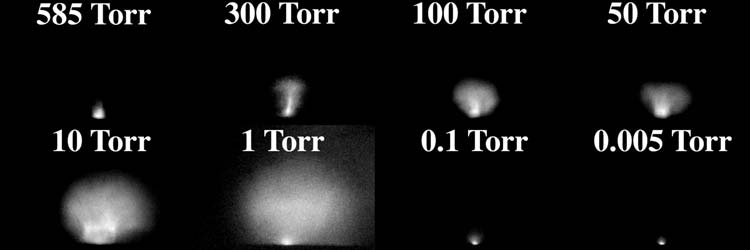
\includegraphics[width = 0.8\textwidth]{chapter_1/plasma_expansion_photo.png}
    \caption[Photo of a plasma expanding.]{ Change in the dimensions of a laser plasma as the air pressure was reduced.}
    \label{fig:plasma_expansion}
\end{figure}
[PHOTO TAKEN FROM LIBS: FUNDAMENTALS AND APPLICATIONS]

The light emitted from the plasma is indicative of the chemical composition of various materials. Positive identification of multiple elemental lines, including both wavelength and intensity within the emission spectrum, contributes to forming a unique spectral fingerprint of the target material. [Fundamentals and applications]
\\
The primary processes that occur during LIBS can be outlined in the following steps:

\begin{enumerate}
\item A short laser pulse is focused on the target material.
\item The incident optical energy is deposited on the sample, resulting in the vaporization of a small amount of its surface.
\item The incoming laser pulse, if its duration is sufficiently large, will also interact with the vapor plume to generate a high-temperature plasma.
\item The system employs a lens or an optical fiber to collect the light emitted from the plasma.
\item A dispersing device, such as a diffraction grating, spatially separates the emitted light into its components. This light originates from the spontaneous emission of hot atoms/ions in the plasma.
\item A digital sensor, such as a CCD or a PMT, is used to collect the light and generate the spectrum.
\item The wavelength and intensity of the resulting atomic emission peaks are analyzed to determine both the chemical elements present in the target sample and their relative concentrations.
\end{enumerate}
Each firing of the laser produces a single LIBS measurement. Typically, however, the signals from many laser plasmas are added or averaged to increase accuracy and precision and to average out nonconformities in sample composition. [LIBS Cambridge]

\begin{figure}[H]
    \centering
    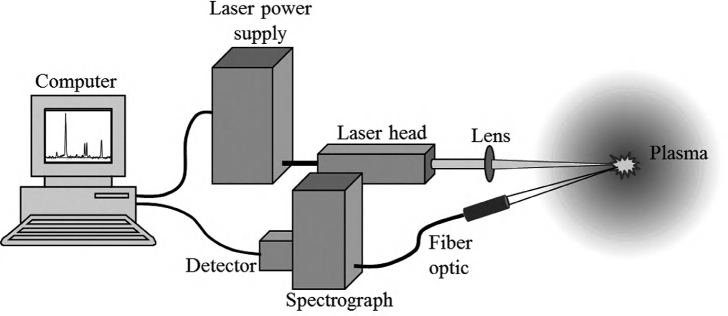
\includegraphics[width = \textwidth]{chapter_1/libs_setup.jpg}
    \caption{A schematic of a general apparatus for laser-induced breakdown spectroscopy illustrating the principal components.}
    \label{fig:libs_setup}
\end{figure}
[PHOTO TAKEN FROM HANDBOOK OF LIBS]

\subsection{Laser-sample Interaction}
\label{subsec:laser-sample_int}

When an atom absorbs a photon, it enters an excited state, where one of its electrons is promoted to a higher energy level. However, the excited states are not very stable, and electrons tend to transition to lower unpopulated energy levels either radiatively, when a photon is generated during the deexcitation process, and non-radiatively when the energy is dissipated in other forms, such as heat or vibration.
\\
Additionally, if the energy applied to the atom is sufficiently high to overcome the ionization potential, electrons can be detached from the atom, creating free negatively charged particles (electrons) and positively charged ions (cations). Initially, the outermost electron, with the lowest ionization potential, is the first to be detached. However, if the supplied energy is high enough, subsequent ionization potentials can be overcome, leading to the detachment of other electrons closer to the nucleus.
\\
There are two main steps leading to breakdown due to optical excitation. The first involves generating a few free electrons that serve as initial receptors of energy through collisions with photons and neutrals. The second is avalanche ionization in the focal region. Free electrons are accelerated by the electric field of the photons, and as the kinetic energy of the electrons grows, collisions will lead to further ionization that will generate even more electrons, creating an avalanche of ionization. 
\\
When a high-energy laser pulse is focused on the surface of a sample, if the irradiance at the focal point exceeds a certain threshold, atoms and ions are ejected from the surface in a process called ablation.

\begin{figure}[H]
    \centering
    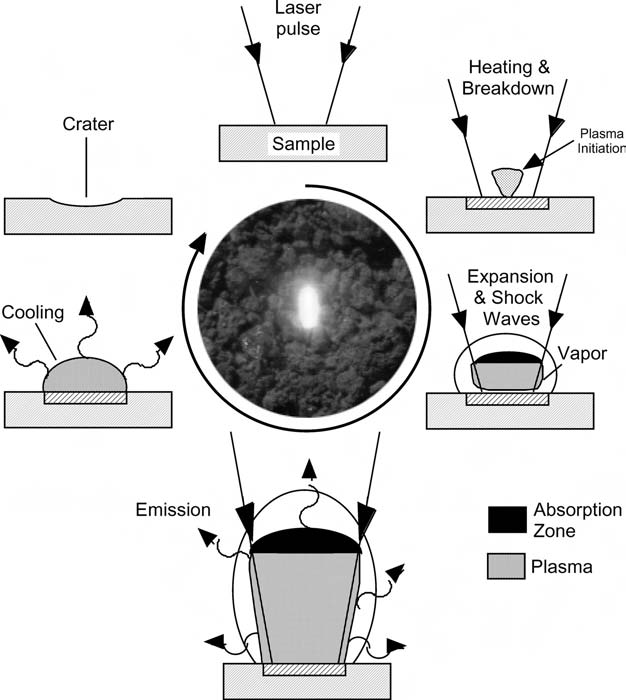
\includegraphics[width = 0.6\textwidth]{chapter_1/libs_life_cycle.png}
    \caption[LIBS life cycle.]{ Life cycle diagram showing main events in the LIBS process.}
    \label{fig:libs_life_cycle}
\end{figure}
[PHOTO TAKEN FROM Fundamentals and Applications]

\subsection{Plasma in LIBS}
\label{subsec:plasma_in_libs}
Given the numerous physical and chemical variables characterizing this state, various definitions of plasma are possible. A plasma can be defined as a local assembly of atoms, ions, molecules, and free electrons, that are overall electrically neutral and exhibit a collective behavior.
\\
Under typical conditions, such as atmospheric pressure and temperature, gases are primarily neutral, with only a marginable amount of charged particles. However, at high temperatures ($T > 1000K$), thermal dissociation of atoms and molecules occurs. Plasma forms when the average kinetic energy of the electrons (given by $k_bT$), significantly surpasses the average binding energy of an electron in an ion.
\\
Plasmas are characterized by a variety of parameters, such as the degree of ionization, the plasma temperature, and the electron density. Depending on the degree of ionization a plasma can be categorized as “weakly ionized”, where the ratio between electrons and other species is less than 10\%, or as “highly ionized” where, on the other hand, atoms could be stripped of many electrons, resulting in a very high electrons-to-ions ratio. LIBS plasmas typically fall in the first category of weakly ionized plasmas; in Figure~\ref{fig:plasma_parameters} we can see how LIBS plasmas compare in temperature and electron density relative to other types of plasma.
\begin{figure}[H]
    \centering
    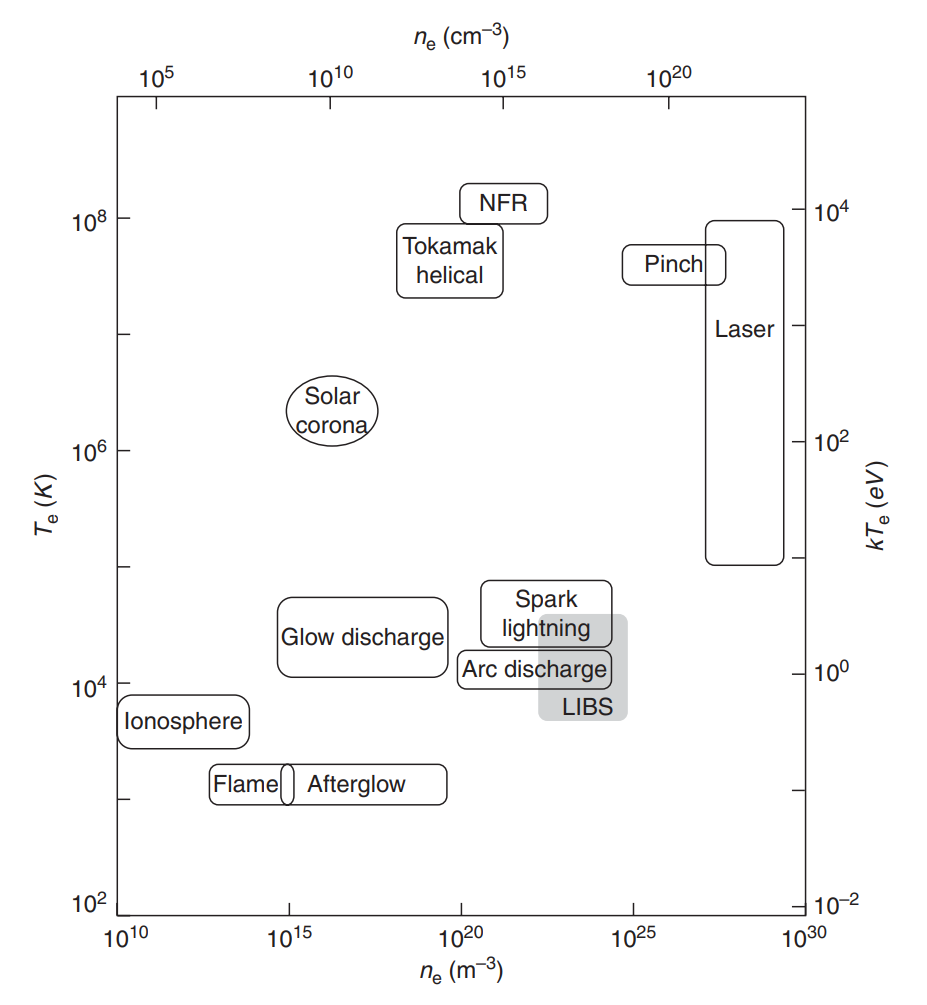
\includegraphics[width = 0.7\textwidth]{chapter_1/plasma_parameters.png}
    \caption{Relation between plasma parameters and type of plasma.}
    \label{fig:plasma_parameters}
\end{figure}
[PHOTO TAKEN FROM HANDBOOK OF LIBS]
The characteristics of the radiation emitted by the plasma depend on the type of radiative transitions that are occurring. At earlier times, where the plasma ionization level is high, the emission will be dominated by a continuum produced by both the bremsstrahlung (free-free transition) and the recombination processes (free-bound transition). Recombination occurs when a free electron is captured by a free ion, releasing its kinetic energy radiatively; while in bremsstrahlung the light is emitted due to electrons being accelerated or decelerated in collisions.
\\
However, the most interesting emissions that can be used for elemental analysis are caused by bound-to-bound transitions that occur between energy levels of ions, atoms, and molecules. 
\begin{figure}[H]
    \centering
    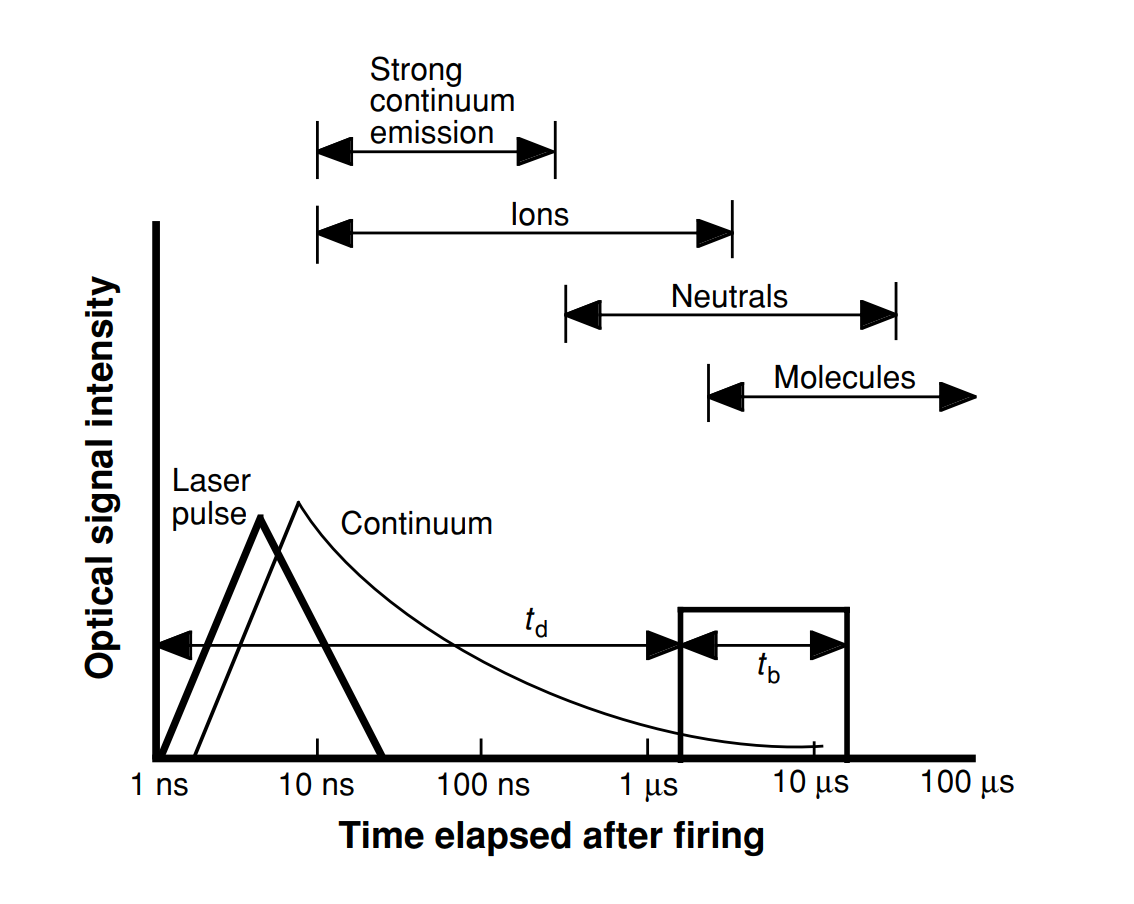
\includegraphics[width = \textwidth]{chapter_1/time_plasma_emission.png}
    \caption{Evolution of the emission of the LIBS plasma over time.}
    \label{fig:time_plasma_emission}
\end{figure}

\subsubsection{Plasma Parameters and Emission Characteristics}
\label{subsubsec:plasma_parameters}
Bound-to-bound transitions are characterized by a fixed energy value, equal to the energy difference between the initial and final level. However, experimentally we see that the measured emission spectrum is not constituted by a collection of sharp lines, but of bell curves instead, with different FWHM. This is because spectral line profiles are also influenced by broadening mechanisms; specifically, pure Doppler broadening, caused by the thermal movement of the emitting particles, will lead to a Gaussian profile, while natural line broadening, due to the time-energy uncertainty principle, and collision broadening will lead to a Lorentzian profile. The collisions between ions and electrons will result in Stark broadening due to the presence of high intensity electric fields near the particles; this phenomenon is predominant in plasmas with higher electron densities, due to the higher probability of collision. 
\\
The Stark broadening causes energy levels to be split according to the value of the quantum number $m_j$, associated with the $z$ component of the total angular momentum $J$, resulting in an asymmetric broadening.
The overall line shape depends on the relative intensity of the different broadening mechanisms and will have a resulting profile obtained by the convolution of the Gaussian and Lorentzian curves, called a Voigt profile.

\begin{figure}[H]
    \centering
    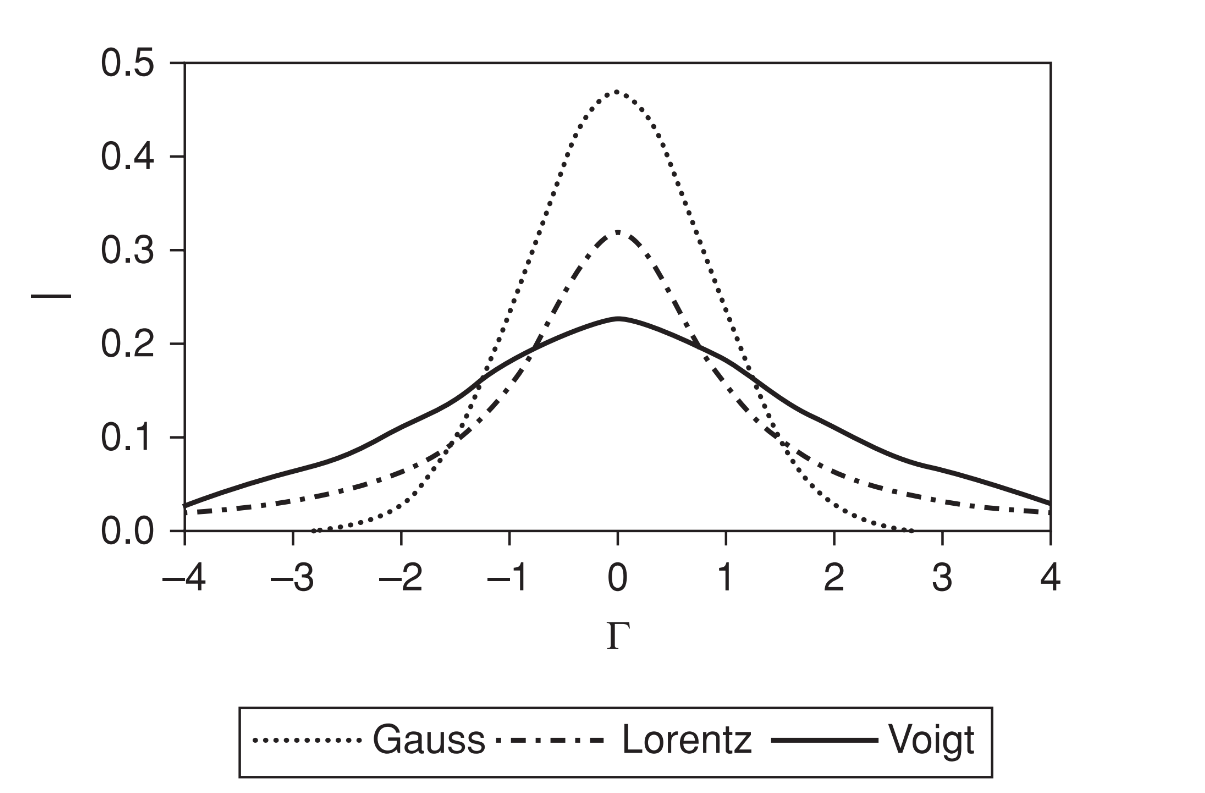
\includegraphics[width = 0.6\textwidth]{chapter_1/voigt.png}
    \caption{Plot of a Voigt profile.}
    \label{fig:voigt}
\end{figure}
[taken from https://scipython.com/book/chapter-8-scipy/examples/the-voigt-profile/]
\\
In normal conditions the main contributions of broadening in a LIBS plasma are due to Doppler and Stark effect. Natural line width is always present but usually the effect is so small that, even without the presence of other broadening mechanisms, it would not be resolved by commonly used LIBS spectrometer ($\Delta\lambda = 0.002\:nm$ for a $10\:ns$ transition at $500\:nm$).
\\
The Doppler width depends only on the temperature of the plasma and on the mass of the particles that are emitting the electromagnetic waves:
\begin{align}
    \Delta\lambda_{D}=7.2\times{10}^{-7}\left(T/M\right)^{1/2}\lambda_{o} \label{eq:doppler_eq}
\end{align}

The Stark effect will produce both a broadening and a shift, and both are dependent on the electron density ($N_e$) and can be used experimentally to obtain the parameter:

\begin{align}
    w_{\mathrm{total}}&\sim\left[1+1.75A\left(1-0.75r\right)\right]\left(n_{e}/{10}^{16}\right)w \label{eq:stark_width} \\ 
    d_{\mathrm{total}}&\sim\left[d/w+2.00A\left(1-0.75r\right)\right]\left(n_{e}/{10}^{16}\right)w \label{eq:stark_shift} 
\end{align}

\subsubsection{Plasma Opacity}
\label{subsubsec:plasma_opacity}
A plasma is defined as “optically thin” when the emitted radiation can freely escape from the plasma without being absorbed or scattered. This is a crucial characteristic to have in a plasma used for LIBS measurement, in this way the emitted radiation can be directly and more easily correlated with the atomic concentrations in the material.
\\
In general, the intensity of the radiation is given by:

\begin{align}
  I\left(\lambda\right)=\left[\varepsilon\left(\lambda\right)/\alpha\left(\lambda\right)\right]\left[1-\exp{\left(-\alpha\left(\lambda\right)L\right)}\right] \label{eq:intensity_radiation}  
\end{align}

Where $\varepsilon$ is the emissivity, $\alpha$ is the absorption coefficient and L is the plasma length in the direction of the observer. For an optically thin plasma we have that $\alpha$ is small and therefore:

\begin{align}
   I(\lambda)=[\varepsilon(\lambda)/\alpha(\lambda)][\alpha(\lambda)L]\varepsilon(\lambda)L \label{eq:intensity_radiation_approx}  
\end{align}

For strong lines, self-absorption will manifest as a flat-topped profile while for other cases certain lines will appear to have a dip in the middle of the curve, in that case the line is called “self-reversed”. 

\begin{figure}[H]
    \centering
    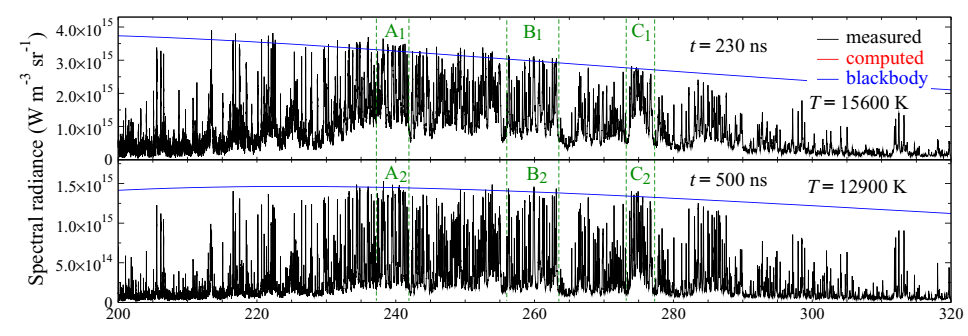
\includegraphics[width = \textwidth]{chapter_1/self_absorption_flat.png}
    \caption{Flat-topped profile of a spectrum caused by self-absorption.}
    \label{fig:self_absorbed_flat}
\end{figure}

\begin{figure}[H]
    \centering
    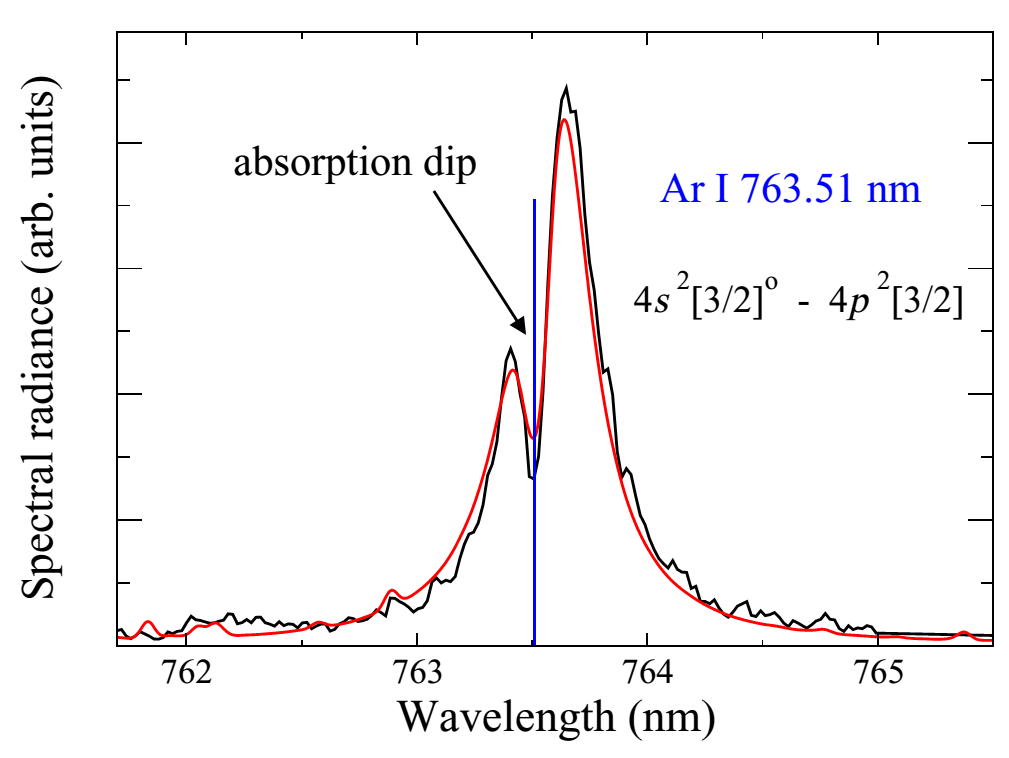
\includegraphics[width = 0.8\textwidth]{chapter_1/self_absorption_peak.png}
    \caption{Self-reversed line caused by high optical thickness.}
    \label{fig:self_absorbed_peak}
\end{figure}
[Taken from jorg's powerpoint]

\subsubsection{Thermodynamic Equilibrium and Plasma Temperature}
\label{subsubsec:thermodynamic_eq}

If a plasma is in thermodynamic equilibrium, it means that all the individual species (electrons, ions, atoms, and molecules) can be described by the same temperature. This condition is generally not true; collisions between particles of the same mass have a much higher probability of equally distributing the kinetic energy after the interaction, this leads to the different species achieving equilibrium individually but not globally, and in general the plasma will be characterized by a different temperature for each one of them.

\begin{figure}[H]
    \centering
    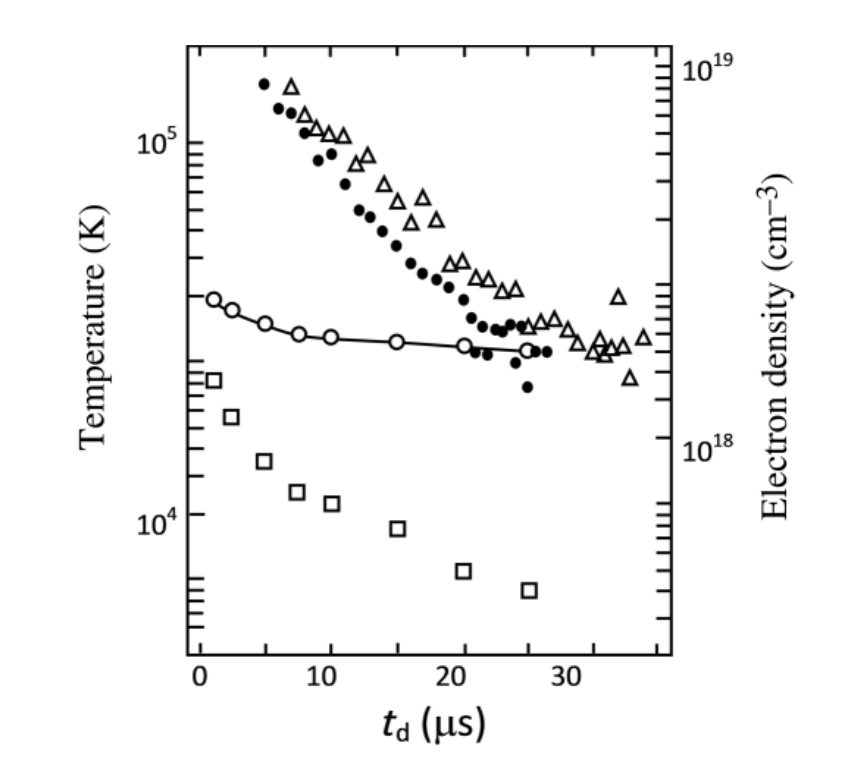
\includegraphics[width = 0.8\textwidth]{chapter_1/electron_equilibrium.png}
    \caption{Convergence of electron temperature for an air plasma.}
    \label{fig:electron_equilibrium}
\end{figure}
[taken from the HANDBOOK of libs]\\
In Figure~\ref{fig:electron_equilibrium} we can see electrons reaching global equilibrium $25\:\mu s$ after the incidence of the pulse. By looking at the Figure~\ref{fig:time_plasma_emission} is evident that the intensity of the emission decays exponentially, and at $25\: \mu s$ the magnitude is already negligible. For this reason, the condition of global thermodynamic equilibrium is not usually required, and it is enough to demand the “Local Thermodynamic Equilibrium” (LTE), where we assume that the equilibrium is reached only locally in small portions of the plasma.
\\
An important criterion to test if a plasma is in thermodynamic equilibrium is the so-called “McWhirter criterion”; is used to see if the electron density is high enough for collision to dominate the population of levels. 
\\
The McWhirter criterion can be expressed by this relation: 

\begin{align}
   n_{e}>1.6\times{10}^{12}T^{1/2}\left(\Delta E\right)^3 \label{eq:mcwhirter_criterion}  
\end{align}
Where $\delta E$ is the energy of the first level above the ground state.
\\
A more precise way to check if the LTE condition is valid is to see if the plasma respects the theoretical temperatures calculated by the Boltzmann and Saha equations. 
For $N_o$ electrons distributed between two levels $i,j$ with respective populations $N_i$ and $N_j$, the relative population will be given by the Boltzmann distribution:
\begin{align}
   N_j/N_{o}=\left(g_j/Z\right)\exp{\left[-E_j/kT\right]}N_j/N_i=\left(g_j/g_i\right)\exp{\left[-\left(E_j-E_i\right)/kT\right]} \label{eq:boltzmann_distribution}  
\end{align}
Where $g_{i,j}$ are the statistical weights and $Z$ is the partition function.
\\
The spectral radial intensity for a given transition with an energy $\lambda$ is then given by: 

\begin{align}
   I=hvAN/4\pi=\left(hcN_0gA/4\pi\lambda Z\right)\exp{\left[-E/kT\right]} \label{eq:spectral_radial_int}  
\end{align}
Where A is the transition probability (Einstein coefficient).
\\
A better and more reliable way to measure the temperature is to use more than one line simultaneously and perform an analysis graphically. By rearranging the previous expression, we obtain:
\begin{align}
   \ln{\left(I\lambda/gA\right)}=-E/kT-\ln{\left(4\pi Z/hcN_0\right)} \label{eq:bolzmann_plot_eq}  
\end{align}

In this way there is a linear dependence between the logarithm of a parameter related to the line intensity and the transition energy, with an angular coefficient $1/kT$. By plotting various transitions of the same element, if the data follows a linear trend, the assumption of LTE is valid, and it is possible to obtain the temperature from the slope.

\begin{figure}[H]
    \centering
    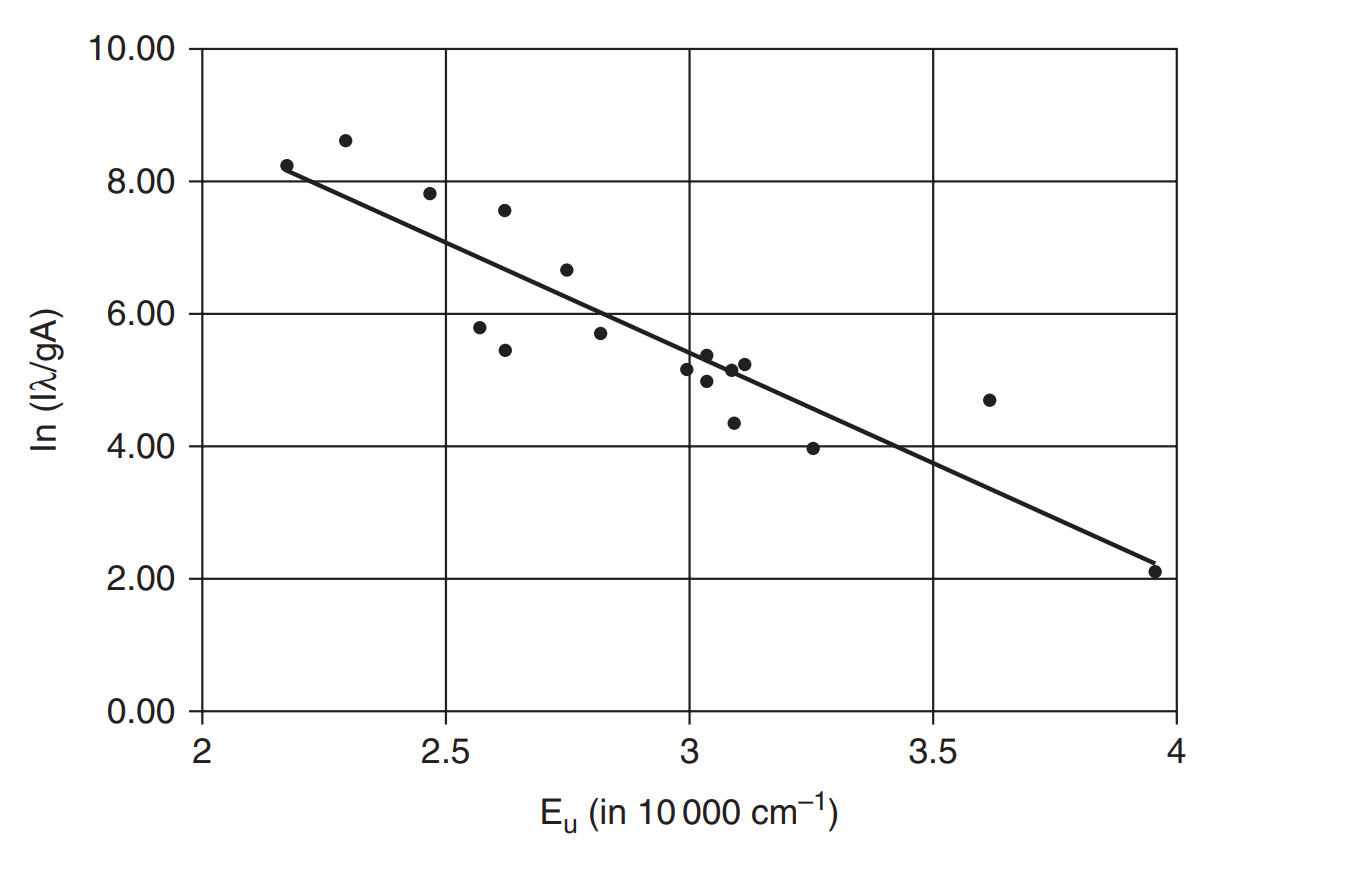
\includegraphics[width = 0.7\textwidth]{chapter_1/boltzmann_plot.png}
    \caption{Multi-line Boltzmann plot based on uranium data.}
    \label{fig:boltzmann_plot_example}
\end{figure}
[taken from the HANDBOOK of libs]\\
While the Boltzmann equation regulates the different populations of energy levels in neutral atoms and molecules, the Saha equation describes the relative populations of different ion stages of a certain atomic species in LTE. The expression of the equation is:

\begin{align}
   \frac{N\left(Z,0\right)}{N\left(Z-1,0\right)}n_{e}=\left(2\left(2\pi m k T\right)^{3/2}/h^3\right)\left(gA\left(Z,0\right)/gA\left(Z-1,0\right)\right)\exp{\left[-\Delta E/kT\right]} \label{eq:saha_equation}  
\end{align}

Where $N(Z,0)$ and $N(Z-1,0)$ represent the population of the ground state of the ion stages $Z$ and $Z-1$ respectively and $\Delta E$ is the ionization energy. It is important to underline that in this case the electron density must be known to apply the expression.
\\
Both equations can be used in conjunction to test for LTE and to estimate the temperature.

\subsection{LIBS Setup Components}
\label{subsec:libs_setup_component}
[taken from Fundamentals and applications]
In a LIBS analysis, four main devices are involved:
\begin{enumerate}
    \item High-energy pulsed laser: Typically operating with nanosecond-duration pulses, the laser is directed at the sample that needs to be studied, causing surface evaporation, and inducing plasma formation.
    \item Spectrometer: Responsible for both diffracting the light collected through an appropriate optical system to obtain its spectral signature and then detecting the intensity of the light at each wavelength. This can be achieved using various devices such as photomultiplier tubes (PMT), photodiode arrays (PDA), or charge-coupled devices (CCD). 
    \item Computer: Processes the acquired spectrum, allowing for further analysis.
\end{enumerate}

Precise time control is crucial in LIBS applications, plasma undergoes various stages in its lifetime that need to be managed to improve the spectral signature.
\\
The selection of the laser, combined with the spectrometer, detector, and time control unit, must be adapted according to the surrounding environmental conditions and the type of materials to analyze.

\subsubsection{Laser}
\label{subsubsec:laser_setup_component}
The laser is the central component of the LIBS system, providing the energy necessary to induce plasma formation. Consequently, the characteristics of the plasma are closely tied to the properties of the laser. The laser influence on the evolution of the plasma occurs both during the interaction between the laser pulse and the sample surface and during the interaction of the laser pulse with the generated plasma plume.
\\
The main parameters related to the laser source include:
\begin{itemize}
    \item Wavelength.
    \item Pulse energy.
    \item Pulse duration (typically in the nanosecond range).
    \item Repetition rate (number of pulses per second) or pulses per measurement.    
\end{itemize}

\paragraph{Wavelength}
\label{par:wavelength_setup_component}
After the initiation of the ablation process, the laser pulse interacts with the gas plume composed of ablated material from the sample's surface. As previously discussed, when the energy of the incoming photon exceeds the bond energy of the electron, photoionization occurs.
\\
Plasma formation primarily occurs through two processes: inverse bremsstrahlung and photoionization. In inverse bremsstrahlung, free electrons gain kinetic energy by absorbing photons from the incident laser light during collisions with atoms and ions.
\\
Inverse bremsstrahlung is more favorable for infrared (IR) and longer wavelengths. [Fundamentals and applications, 26] Consequently, laser sources with shorter wavelengths transfer energy to the material more efficiently, leading to higher ablation rates since the effect of plasma shielding is lower. However, for the same reason plasma ignition is less efficient with shorter wavelengths, resulting in a higher threshold for plasma formation. On the other hand, longer wavelengths will transfer energy to the plasma more efficiently but resulting in lower surface ablation.
\\
A variety of lasers are utilized in LIBS systems, with solid-state Nd: YAG lasers being commonly employed. This choice is attributed to their relatively low cost, ease of maintenance, and compact size, enabling their integration into systems of various sizes. The Nd: YAG laser typically operates at a fundamental wavelength of $1064\:nm$ with a pulse temporal width between $6$ and $15\:ns$. However, it is common for these lasers to operate at higher harmonics, such as the second harmonic at $532\:nm$, the third harmonic at $355\:nm$, or the fourth harmonic at $266\:nm$. These higher harmonics are less powerful and feature shorter pulse durations, typically between 4 and $8\:ns$ [Fundamentals and Applications].

\paragraph{Pulse Energy}
\label{par:pulse_energy_setup_component}
Both ablation and plasma ignition are significantly influenced by the energy and temporal duration of the laser pulse. In LIBS applications, the energy delivered to the sample per unit area is a more critical parameter than the absolute energy value of the laser pulse. Therefore, the primary physical quantities used in the analysis are Fluence, which represents energy per unit area (measured in $J/cm^2$), and Irradiance, which represents power per unit area (measured in $W/cm^2$).
\\
For this reason, fluence and irradiance can be adjusted both by varying the energy of the pulse and by tuning the focal length of the system, in order to change the spot size of the laser on the sample surface.
\\
Variations in pulse energies and focusing distances will also impact the shape and temporal evolution of the plasma plume [Analytical Chemistry LIBS]. At high irradiances, the plasma will contain more ablated material and possess greater internal energy, allowing it to expand with a hemispherical shape by pushing the surrounding air farther away. Conversely, at lower fluence levels, the plume will expand with less energy, resulting in a shape similar to a disk that evolves radially and remains closer to the surface of the sample.
\paragraph{Laser Pulse Duration}
\label{par:laser_pulse_duration_setup_component}

Regardless of their duration, laser pulses typically meet the necessary conditions for ablating targets. The rate of energy deposition will, indeed, surpass the rate of energy redistribution and dissipation through the sample lattice, leading to extremely high temperatures in those regions where energy absorption occurs.
\\
The nature of ablation is strongly influenced by the duration of the laser pulse.
When using lasers that generate pulses in the femtosecond regime, non-thermal processes dominate the ionization. This means that since the pulse duration is too short to induce thermal effects in the sample's matrix structure, other mechanisms are therefore responsible for ionizing the atoms. In this case, the pulse carries a significant amount of energy, and phenomena such as photochemical absorption, multi-photon absorption, tunneling, and avalanche ionization occur to excite the sample. 
\\
The absence of thermal effects results in the formation of a crater with sharply defined edges, without any melted or deposited materials surrounding it. After the laser pulse, only a very hot electron gas and an essentially undisturbed lattice remain.
\\
Conversely, when using laser pulses in the nanosecond regime, different effects come into play. The time required for electron-lattice heating is approximately $1\:ps$ [Fundamentals and Applications], much shorter than the duration of the pulse. As a result, thermal effects dominate the ionization process.
\\
After the interaction with the laser pulse, the material undergoes transient changes in thermodynamic states, transitioning from solid to liquid and ultimately into a plasma state [Analytical Chemistry].
\\
In simple terms, the pulse initially melts and vaporizes the surface, with the increasing temperature eventually leading to the ionization of atoms. If the irradiance is sufficiently high, both thermal and non-thermal effects will contribute to the ionization of the sample. Between 1 and $10 \: ns$, the plasma becomes opaque to laser radiation [Fundamentals and Applications]. As a result, the latter part of the pulse does not significantly contribute to surface vaporization. Instead, it interacts with the already generated plasma plume, potentially being absorbed, or reflected. This interaction leads to a decrease in the ablation rate, a phenomenon known as "Plasma Shielding." 
\\
Plasma Shielding is highly dependent on environmental conditions such as pressure and the composition of gases in the atmosphere, as well as experimental factors including laser wavelength and irradiance.
\\
When using nanosecond pulses, the generated craters typically exhibit melted and deposited material around them, as seen in the SEM images shown in Figure~\ref{fig:craters_laser_duration}:
\begin{figure}[H]
    \centering
    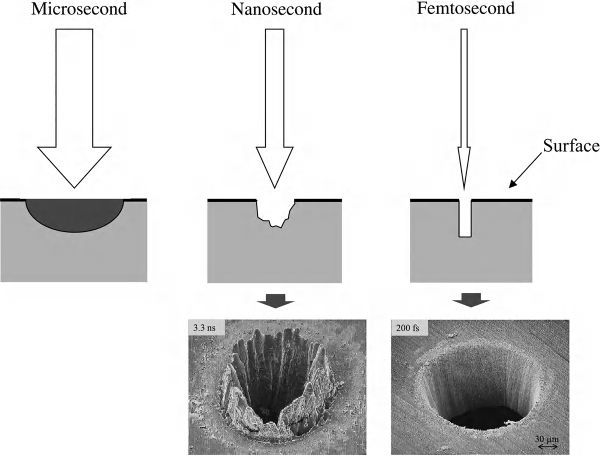
\includegraphics[width = 0.7\textwidth]{chapter_1/craters_laser_duration.jpg}
    \caption{SEM images of craters produced by different types of laser.}
    \label{fig:craters_laser_duration}
\end{figure}
[taken from the HANDBOOK of LIBS]
\\
At the same time, the plasma is reheated, resulting in longer plasma lifetimes and larger plasma plume sizes [Fundamentals and Applications].
\subsection{Spectra Evaluation}
\label{subsec:spectra_evaluation}
Once the plasma has been ignited, the emitted light is collected by a detector, which creates a spectrum with the intensities of the measured light on the $y$ axis, and the wavelengths on the $x$ axis. 
\begin{figure}[H]
    \centering
    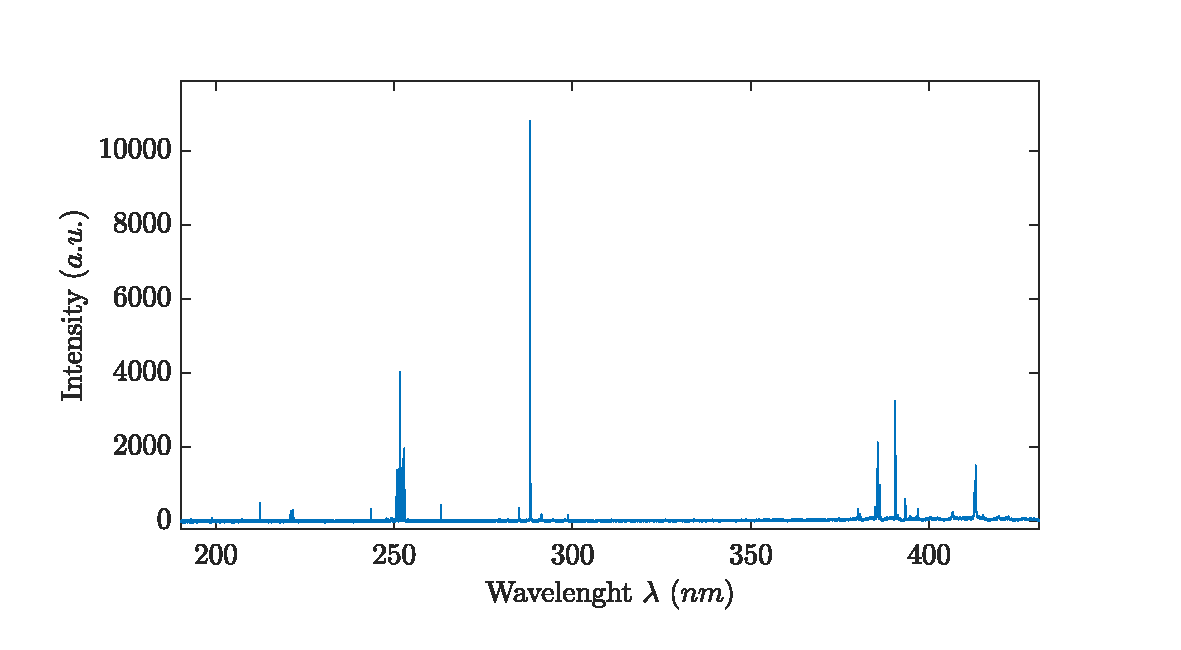
\includegraphics[width = \textwidth]{chapter_1/generic_spectrum.pdf}
    \vspace*{-30pt}
    \caption{LIBS spectrum of a pure silica sample we measured.}
    \label{fig:generic_spectrum}
\end{figure}
This spectrum may contain emission lines from atomic species, as well as continuous radiation resulting from bremsstrahlung [Fundamentals and Applications].
\\
Continuous radiation can hide emission lines, so efforts should be made to minimize its detection. 
\\
Since the energy of a transition is characteristic of the particle species, analyzing photon energies can reveal the composition of the plasma.
Accurate identification of LIBS emission lines is essential for determining the elemental constituents of a sample. The analysis of the LIBS spectrum will reveal elements present at concentrations above the method's minimum detectable limit (LOD).
\\
The most important spectral region for LIBS typically spans from 200 to $800\: nm$, where most elements exhibit strong emission lines. In addition to emission from atoms and ions, emission from simple molecules may also be observed in the samples. Generally, high concentrations of the elements composing the molecules must be present for molecular emission to be observed.
\\
Currently, LIBS is limited by problems of low reproducibility, with a resulting poor accuracy. Problems associated whit shot to shot variations in plasma conditions, which are caused by the stochastic nature of the laser source and light-matter interaction, seem to be the major cause of this effect [Applications of single-shot laser]. For this reason, a single measurement is usually obtained by averaging hundreds of different shots.
\\
More details on spectra evaluation will be presented in %Chapter~\ref{}

\chapter{Glass Manufacturing}
\label{ch:experimental_techniques}

\section{Grinding of Glass}
\label{sec:grinding_glass}

The manufacturing process of polished glass pieces typically begins with grinding, which, thanks to its ability to achieve surface flatness while maintaining high MRRs on hard and brittle materials, is considered one of the most important and feasible machining technologies. However, grinding can induce surface and subsurface damage on the glass sample. Consequently, chemical mechanical polishing (CMP) is employed to eliminate these residual defects [CMP of glass disk].
\\
Grinding too is a complex process, especially when applied to glass due to the nature of the material. The most used abrasive materials are silicon carbide or diamond grinding wheels [Grinding of Glass: the mechanics of the process *(GoG)*]. 
\\
Previous research shows that both permanent viscous flow and brittle fracture can occur during the grinding of glass surfaces. 
Viscous flow is the main grinding mechanism when using silicon carbide. On the contrary, when using diamond grinding wheels, glass is ground mostly through brittle fracture of particles from the surface.

\subsection{Non-Newtonian Flow of Glass Particles}
It is widely recognized that glass can be made to flow without fracturing under significant hydrostatic compressive stresses, even at ambient temperature [GoG]; this can happen because the local surface temperature in the grinding zone can easily exceeds the glass's softening point. The pressure conditions, favorable for the flow of glass, are also expected to exist at the cutting edge of an abrasive grain during grinding.
\\
It has also been observed that most of the grinding energy is dissipated in the material by viscous deformation [GoG]. For this reason, glasses with high softening temperatures also have a high specific grinding energy, that is defined as the proportionality constant between the work expended in the process and the rate of material removal.
\\
Additionally, it has been observed that there is a correlation between the increase in specific grinding energy and the decrease in particle grain sizes [GoG].
\\
Numerous experimental investigations have clearly demonstrated that when soda-lime glass is subjected to sufficiently high axial stress or pressure, it exhibits a nonlinear mechanical response, and an irreversible deformation takes place, a phenomenon known as inelasticity or material nonlinearity [Material Nonlinearity and Inelasticity] [non-Newtonian viscous flow]. Studies of the viscosity of stable soda-lime glass under high shear stress have revealed a non-Newtonian viscosity of the pseudoplastic type. In this behavior, if the applied stress rate exceeds a certain threshold value, catastrophic failure of the material occurs, leading to the formation of numerous cracks and an eventual brittle fracture of the glass sample [Non-Newtonian Viscous Flow].
\\
The interpretation of this non-Newtonian behavior is attributed to atomic structural rearrangements within the glass material. These rearrangements play a significant role in determining the material's mechanical response under high stress conditions, ultimately influencing its flow and fracture characteristics during the grinding process.
\section{Chemical Mechanical Polishing}
\label{sec:CMP}
Chemical mechanical polishing (CMP) has been a widely used planarization method in various industries, including integrated circuits manufacturing and glass surface polishing, for many decades. The effectiveness of CMP in achieving planar, smooth, and damage-free surfaces is influenced by numerous factors related to the sample carrier structure, polishing pad, slurry composition, and other process parameters. Since both chemical and mechanical actions play a role in CMP, and since they are influenced by multiple variables, understanding the complexity of the CMP mechanism is still a great challenge and is an actively researched topic.
\\
CMP aims to produce planar surfaces on target materials by removing micro and nano-sized particles, sometimes acting even on the atomic-scale; with the goal of achieving sub-nanometer level roughness while minimizing surface and subsurface damage [CMPTE]. The surface smoothing effect observed in CMP is attributed to various mechanisms, including the non-Newtonian flow of glass material, fretting and mechanical abrasion caused by friction between the glass and the polishing tool, and chemical reactions leading to surface decomposition.
\\
In general, mechanical abrasion and chemical removal are typically the predominant mechanisms, leading to the use of the term: "chemo-mechanical polishing" [Gerhard et al. Appl Surf Sci].
\\
Mechanical removal is mostly based on the interaction of the glass surface with abrasive grains, such as cerium oxide or aluminum oxide, present in an aqueous polishing slurry. On the other hand, chemical removal involves complex processes such as diffusion of water molecules into the glass sample, redeposition of silica on the surface during polishing, and diffusion of polishing agents into the surface of the glass [Cook, 1990].
\\
Polishing is not only needed to obtain a transparent surface of an optical glass component with the required accuracy, but also to remove digs, pits, and microcracks induced by the previous processes to obtain smooth surfaces that minimize scattering [Optics Manufacturing (Gerhard)].

\subsection{CMP Technique}
\label{subsec:cmp_technique}

Chemical mechanical polishing (CMP) is a process that, by definition, combines chemical and mechanical actions to enhance the material removal rate (MRR), which quantifies the amount of material removed per unit time. The MRR is influenced by various factors including the system configuration, the properties of the abrasive pad, and the composition of the polishing suspension employed.
\\
Depending on the layout of the polishing machine, different approaches and principles can be applied for polishing.
\\
There are four main types of commercially available CMP equipment commonly used in industry, as shown in Figure~\ref{fig:cmp_equipment}: 
\begin{figure}[H]
    \centering
    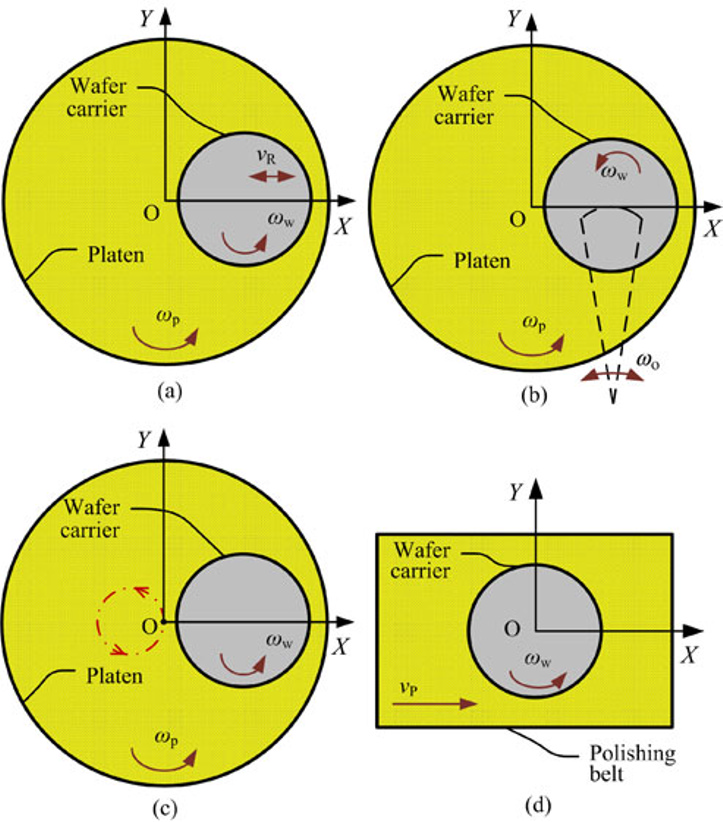
\includegraphics[width = 0.4\textwidth]{chapter_2/cmp_equipment.png}
    \caption[Schematic of different types of CMP equipment.]{ Schematic of different types of CMP equipment: (a) rotary type, reciprocation mode, (b) rotary type, oscillation mode, (c) orbital type, and (d) linear type.}
    \label{fig:cmp_equipment}
\end{figure}
[taken from CMP theory and experiments]

\begin{enumerate}
    \item Rotary type polisher with a sample carrier featuring a reciprocating motion along the platen diameter.
    \item Rotary type polisher with a sample carrier exhibiting an oscillatory motion.
    \item Orbital type polisher with the platen having an orbital rotation.
    \item Linear type polisher equipped with a linear motion belt as the polishing pad.
\end{enumerate}
The movement of the carrier and the platen generates the necessary relative motion for the polishing process, while a slurry, containing particles and chemical solutions, is delivered onto the pad to act as the abrasive [CMPTE]. Through the combined chemical actions of the solutions and the mechanical actions of the particles, micro material removal occurs, enabling surface polishing and finishing to be realized.
\\
The MRR, non-uniformity, and surface quality are key indicators of machining and CMP process efficiency. These parameters are influenced by some major factors such as the system configuration, process variables (e.g., down pressing force of the sample on the pad, relative velocity of the pad), and consumables (e.g., slurry concentration). The synergetic interaction of these input variables determines the final polishing results by affecting the sample-pad interaction and material removal process. 

\subsection{Modeling of CMP}
The removal rate in CMP is determined by several parameters at the sample-pad interface, including pressure, temperature, and slurry distribution over the active surface. Many process variables, such as sample pressing downforce, pad rotation speed, slurry characteristics and the employed pad material, can influence the final polishing outcomes [CMPTE].
\\
A theoretical description of the polishing of optical glasses is thus a complex task since such polishing processes are based on different interacting mechanisms. These different mechanisms have been described by some models: the removal, the flow, the chemical, and the fretting hypothesis [Optics Manufacturing (Gerhard)].
\\
Under the removal hypothesis, the sharp edges of the abrasive particle grains of the polishing agent enter in contact with the surface of the glass digging out small particles. Since these interactions preferentially target the roughness peaks of the working surface, a smoothing effect is obtained over time [Optics Manufacturing (Gerhard)].
\\
The flow hypothesis says that in addition to the mechanical removal by abrasion, the polishing agent grains also perform an irreversible displacement of the glass material. Here, due to the friction between the work piece surface and the polishing pad and grain, the local temperature can rise above the softening point of the glass and as a result, roughness peaks are dislocated into roughness valleys or digs by material flow. 
\begin{figure}[H]
    \centering
    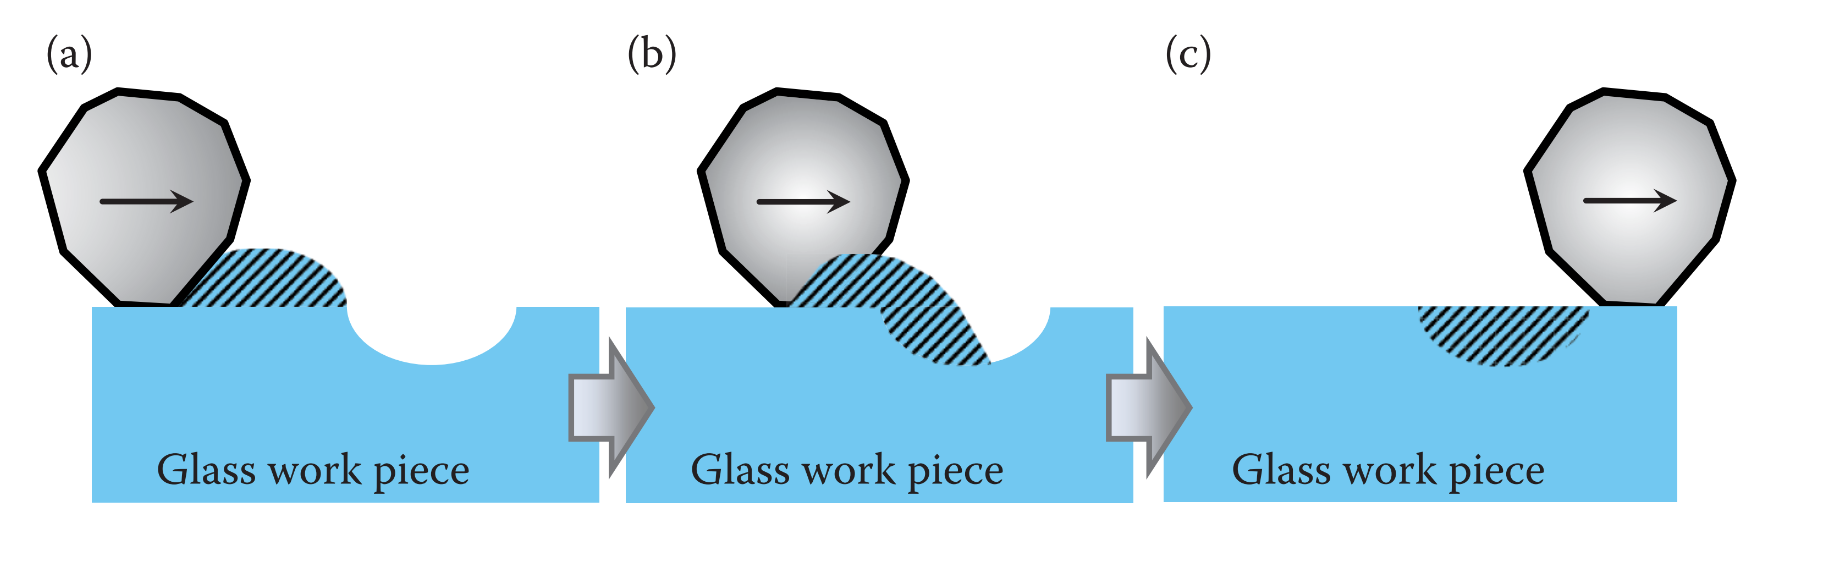
\includegraphics[width = \textwidth]{chapter_2/flow_hypothesis.png}
    \caption[Visualization of the flow hypothesis.]{ Visualization of the flow hypothesis; roughness peaks (dashed structure) are softened by wear in the course of the polishing process (a) and dislocated into roughness valleys or digs (b), consequently resulting in a leveling of the surface (c).}
    \label{fig:flow_hypothesis}
\end{figure}
[image taken from optics manufacturing Gerhard]
Under the chemical hypothesis are described the chemical reactions that take place on the surface of the target glass sample. Such reactions are supported by hydrolytic scission of bonds of the glass network [Optics Manufacturing (Gerhard)] according to Equation~\ref{eq:hydrolytic_scission}:
\begin{align}
\ce{(SiO2)_x + 2H2O <-> (SiO2)_{x-1} + Si(OH)4} \label{eq:hydrolytic_scission}
\end{align}
The rate of the reaction is controlled by the diffusion of water molecules at the surface of the glass [Cook, 1990]. The depth of this diffusion layer can be estimated, after a given time “$t$”, by the relation: 
\begin{align}
    d_{dif}\ \approx\ 2\sqrt{Dt} \label{eq:diff_length}
\end{align}
Where D is the diffusion coefficient of water into glass and its value can range from $10^{-15} \:cm^2/s$ to $10^{-18}\: cm^2/s$ : (Nogami and Tomozawa, 1984; Lanford et al., 1985).
\\
As a result of this phenomenon, hydrated silica is deposited on the sample surface during polishing, consequently leading to the formation of a silica gel layer [Optics Manufacturing (Gerhard) (Iler, 1979; Cumbo and Jacobs, 1994)] that contributes to surface smoothing, since it can accumulate in digs and scratches filling those geometric surface defects. 
\\
The last studied mechanism is based on the material removal due to fretting, arising from the synergy between two physical factors: the contact pressure of the polishing tool on the glass surface and their relative movement [Optics Manufacturing (Gerhard) (Dimatteo, 1997)]. This early model, developed by Frank W. Preston in the late 1920 (Preston, 1927) describes the MRR through an empirical equation as follows:
Formula (8.4) in [Optics Manufacturing (Gerhard)] and [CMPTE]
\begin{align}
    MRR=kPV \label{eq:material_removal}
\end{align}
Here, “$k$” is an empirical constant determined from experimental data, P is the pressure applied to the sample and $V$ is the relative velocity between the glass and the polishing tool.
\\
This equation only considers the mechanical contributions to the MRR, neglecting the chemical actions. In this way, the polishing process can be described as a simple two body wear problem, where the target sample is pressed down on a polishing pad and moving at a fixed speed.
\\
To increase the accordance with experimental data, an alternative expression for the Preston equation have been proposed: $MRR=kP^\alpha V^\beta$[CMPTE]; where the dependence of the $MRR$ relative to the pressure and velocity is no longer linear. However, this model still fails to correctly describe processes where chemical interactions are crucial.

\section{Polishing Elements}
\label{sec:polishing_elements}
In the polishing process a resilient pad, a target sample to be polished, and an abrasive slurry are the key components. The process involves pressing a glass sample face down onto a rotating polishing pad while a slurry containing abrasive particles and chemical additives flows between them. This mechanical and chemical action removes material from the sample, resulting in a smoother surface.
\subsection{Polishing Pad}
Different types of pads can be utilized for polishing, even though traditionally the typical polishing pad was made of pitch [Optics Manufacturing (Gerhard)], a natural viscoelastic polymer, also known as bitumen or asphalt, derived from petroleum or tar. Today polishing pads are typically made of porous polyurethane [CMPTE] with additional components added to tune the pad hardness [CMPTE 4]. This material is capable of higher process velocities, and it is less sensitive to temperature changes [Optics Manufacturing (Gerhard)]. 
\\
The hardness of the pad is a critical property that can influence both the material removal rate (MRR) and the uniformity of polishing [CMPTE]. Different applications and types of target materials may require either hard or soft pads.
\\
Both the bulk of the pad and the surface are full of micropores, which are useful for retaining the abrasive particles of the slurry; these micropores play a crucial role in the polishing process by facilitating the interaction between the pad, the slurry, and the sample. As shown in Figure~\ref{fig:hard_soft_pad}
\begin{figure}[H]
    \centering
    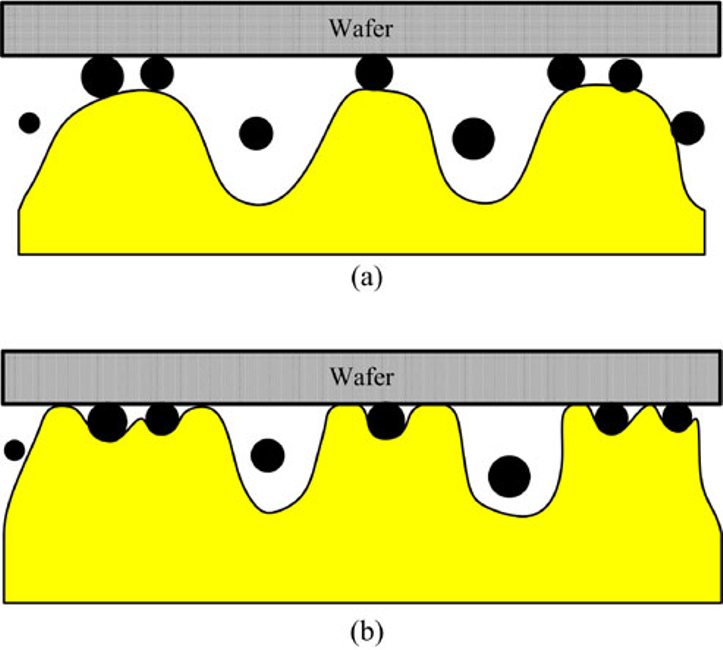
\includegraphics[width = 0.6\textwidth]{chapter_2/hard_soft_pad.png}
    \caption[Comparison between a hard pad and a soft pad.]{ Contact status of (a) hard pad, and (b) soft pad. }
    \label{fig:hard_soft_pad}
\end{figure}
During CMP, the physical properties of the pad, such as hardness and surface roughness, are expected to change due to mechanical loads and chemical reactions occurring during the polishing. These changes could significantly impact the process, so they should be limited to ensure consistent results.

\subsection{Polishing Suspension (Slurry)}
\label{subsec:polishing_slurry}

The slurry used in CMP is a complex mixture consisting of abrasive materials dispersed in water along with various chemicals, including oxidants, inhibitors, and bases to adjust the pH. Abrasive particles such as \ce{SiO2}, \ce{CeO2}, and \ce{Al2O3}, with sizes ranging from 10 nanometers to some micrometers [Optics Manufacturing (Gerhard)], are commonly used in industrial CMP processes. The mass concentration of the polishing agent relative to the total slurry usually spans from 5\% to 30\% [Bliedtner and Gräfe, 2008].
\\
The choice of a particular polishing agent depends on the material of the work piece [Optics Manufacturing (Gerhard)], while the properties of the abrasive particles, such as the size distribution, chemical composition, and concentration, as well as the pH of the slurry, will have a significant impact on the material removal rate ($MRR$), uniformity, and surface quality of the polished material [CMPTE]. For example, at pH values of 3.0 and 10.0, the material removal is primarily driven by chemical corrosion, while at a pH around 7.0, the mechanical action of abrasive particles becomes the dominant factor contributing to the $MRR$. [Effects of chemical additives of CMP]
\\
During CMP, the slurry plays a crucial role at the interface between the wafer and the polishing pad. The flow of slurry brings abrasive particles and chemicals to the interface, where they initiate the polishing process by removal or material flow [Optics Manufacturing (Gerhard)]. The slurry will form a lubricating film, reducing friction forces between the wafer and pad, and the fluid presence can also help support some of the downforce, thereby relieving pressure from the pad [CMPTE].
\\
Physical models have shown that in slurry with a size distribution of abrasive particles, only the larger particles make direct contact with the pad and the sample, leading to effective material removal [Effect of chemicals on CMP of glass substrates]. 

\section{Side Effects of Polishing}
\label{sec:polishing_side_eff}

The uniformity of glass substrate surfaces in terms of index of refraction, chemical composition, and roughness is crucial in many different applications. However, during the manufacturing process, from rough grinding to fine polishing, nonuniform surfaces can arise. This is due, for example, to the presence of contaminants inside the glass, caused by residues of operating materials used during manufacturing as, most commonly, polishing agents.
\\
One significant chemical mechanism, happening on the surface of the sample during CMP, is the formation of a silica gel layer, also known as the redeposition layer [Gerhard et al appl opt 2017].
\\
This layer forms as water penetrates the glass surface, leading to hydrolytic scission of the glass network, which results in the formation of a thin layer consisting of hydrated silica, or silanol. During the growth of this layer on the surface, also known as Beilby layer, residues from polishing agents and other elements from the polishing suspension can remain embedded within it [Gerhard et al appl surf sci].
\\
For example, some studies [Kozlowski] have shown that aluminum from corundum-based abrasives can exceed a mass fraction of 1000 ppm on the glass surface. This retention occurs as particles from the polishing slurry accumulate within surface defects such as digs, scratches, and microcracks formed during earlier manufacturing steps [Gerhard et al Appl Opt 2017].

\begin{figure}[H]
    \centering
    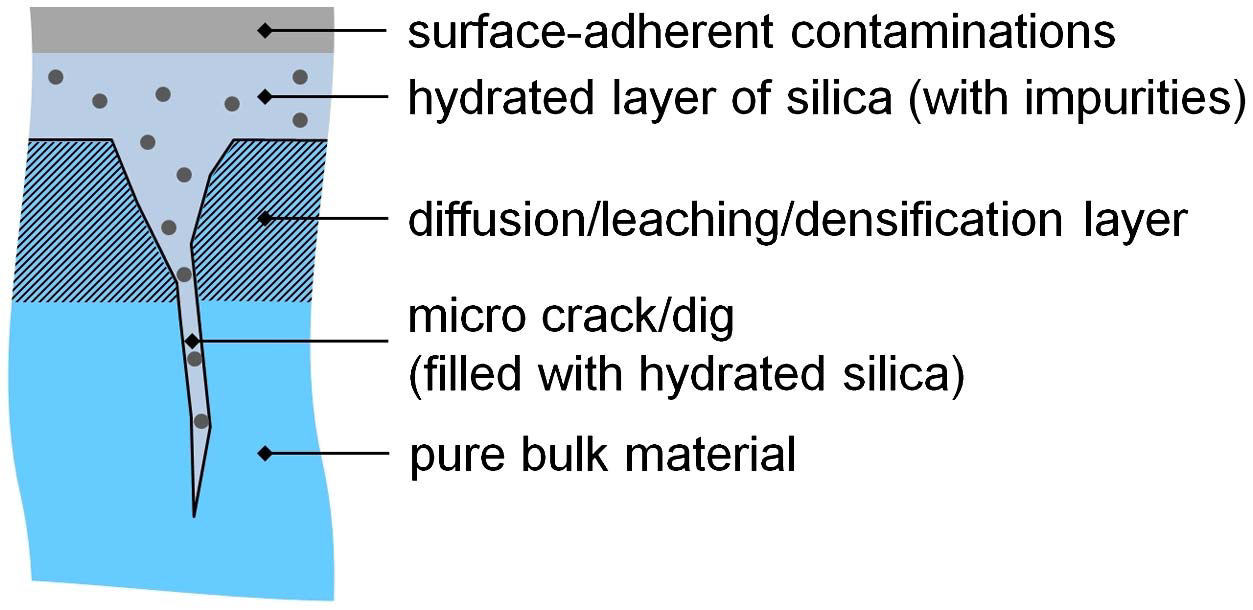
\includegraphics[width = 0.6\textwidth]{chapter_2/micro_cracks.png}
    \caption[Schematic of a surface defect generated during optics manufacturing.]{ Schematic presentation of a typical surface defect generated
during classical manufacturing of optical surfaces. }
    \label{fig:micro_cracks}
\end{figure}
[taken by Gerhard app optics]
\\
As a result of these processes, visually clean polished glass surfaces can exhibit significant optically active contaminations [Gerhard et al Appl Opt 2017]. These contaminations may include surface adherent contaminants such as hydrocarbonaceous compounds and residues from polishing agents. The remaining silica gel layer and contaminants on the surface can also lead to negative effects such an increase in near-surface absorption consequently lowering the laser-induced damage threshold [Optics Manufacturing (Gerhard)].

\section{Diffusion}
\label{subsec:diff}

As already mentioned in Chapter~\ref{sec:CMP}, diffusion is a core process in optics manufacturing; following is a brief exposition on the main characteristics of the mechanism.
\\
Diffusion is a physical and time dependent mechanism that drives the flow of particles from a low concentration portion of a medium to a high concentration one. The process is purely thermodynamical, the difference between the chemical potential, i.e. the potential associated with the concentration of particles, causes a difference between the Gibbs free energy of the two areas and leads to the flow of material in order to achieve equilibrium.
\begin{figure}[H]
    \centering
    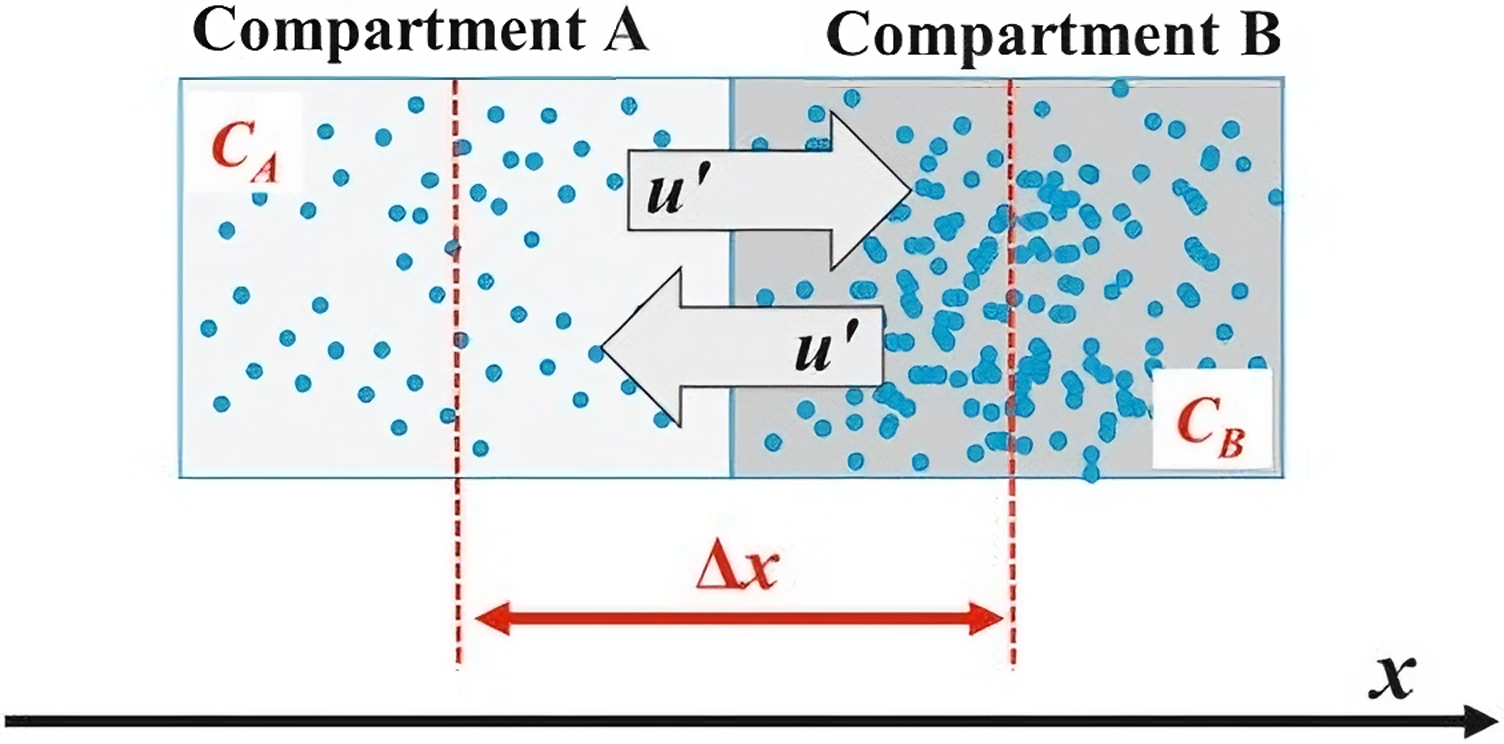
\includegraphics[width = 0.5\textwidth]{chapter_2/diffiusion_upscaled.jpg}
    \caption[]{Diffusion driven by the difference in concentration in the two compartments.}
    \label{fig:diff_drawing}
\end{figure}
[taken by https://www.sciencedirect.com/topics/earth-and-planetary-sciences/molecular-diffusion]
The simplest diffusion processes are called “normal” (or “Fickian”) and can be modelled by the two Ficks’s laws. 
\\
The first one is:
\begin{align}
    \vec{J}=-D\vec{\nabla}C \label{eq:first_law_3d}
\end{align}
Where the vectorial flow of particle $\vec{J}$ is proportional to the gradient of the concentration with a proportionality constant “$D$”, which is called diffusion coefficient. This coefficient, in general, will depend on both the substrate and the species diffusing into it, as well as on other external parameters like temperature and pressure. 
\\
It is very common to model diffusion processes one dimensionally, the first Fick’s law then becomes:
\begin{align}
    J=-D\frac{\partial C}{\partial x} \label{eq:first_law_1d}
\end{align}
Where we can clearly see that without any difference in concentration along x there is no flow of particles.
\\
The first law only describes the spatial dependence of the process. To also introduce the time dependency, it is necessary to also consider the second Fick’s Law, which states:
\begin{align}
   \frac{\partial C}{\partial t}=D\nabla^2C \label{eq:second_law_3d}
\end{align}
Under a 1-D approximation Equation~\ref{eq:second_law_3d} becomes:
\begin{align}
   \frac{\partial C}{\partial t}=D\frac{\partial^2C}{\partial x^2} \label{eq:second_law_1d}
\end{align}
Where the same proportionality constant D relates the concentration derivative with respect to time to its second spatial derivative.
\\
This partial differential equation can be solved by taking as boundary condition a fixed concentration $C_0$ at a certain value of $x$ (usually $x = 0$). This models a situation where a constant source of external diffusant is applied at one of the surfaces of a material.
\\
The solution of the equation, which is only valid for positive values of $x$, is:
\begin{align}
    C\left(x,t\right)=C_0\operatorname{erfc}\left(\frac{x}{2\sqrt{Dt}}\right) \label{eq:fick_solution}
\end{align}
Where $\mathrm{erfc}$ is the complementary of the error function and is defined as:
\begin{align}
   \operatorname{erfc}z=1-\frac{2}{\sqrt\pi}\int_{0}^{z}e^{-t^2}\ dt 
\end{align}

\begin{figure}[H]
    \centering
    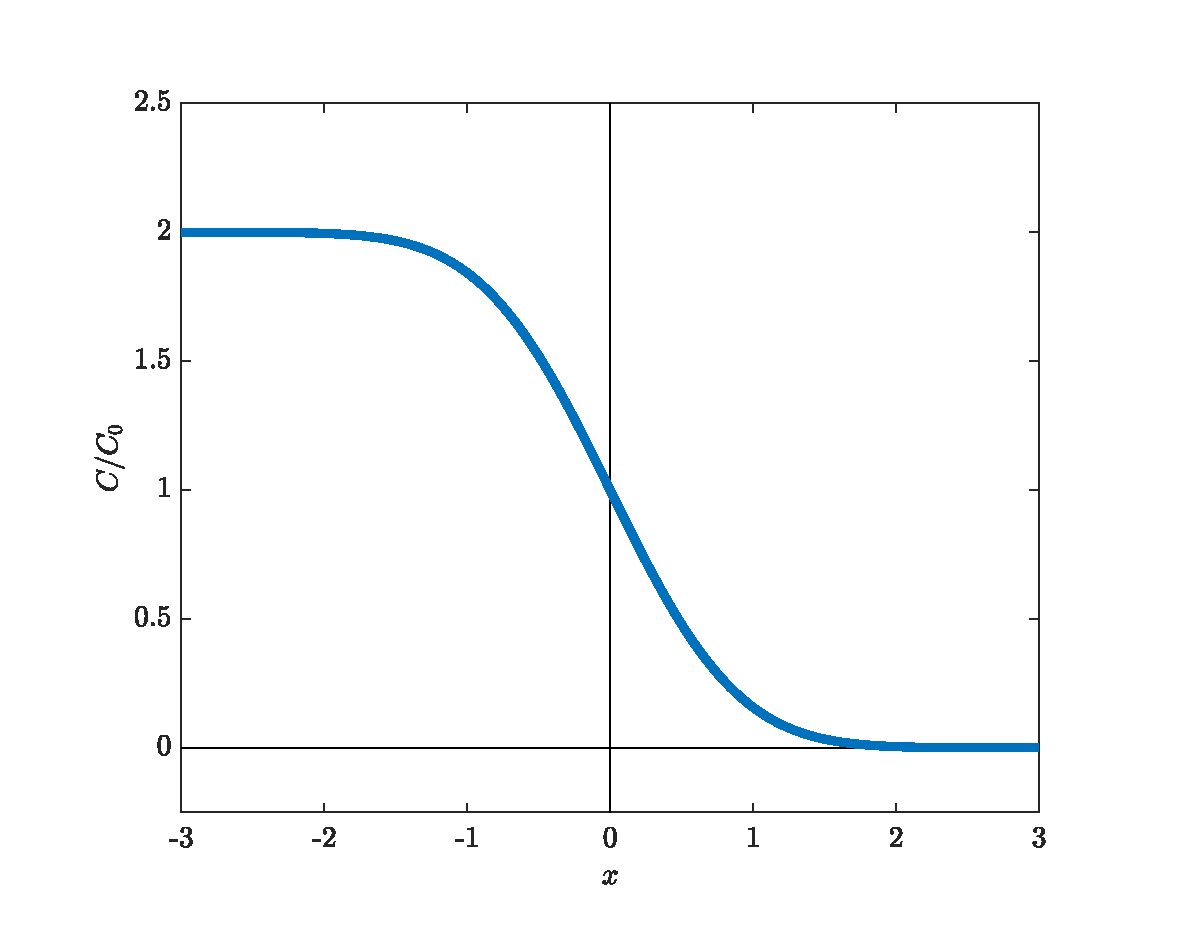
\includegraphics[width = \textwidth]{chapter_2/plot_erfc.pdf}
    \vspace*{-40pt}
    \caption[]{Plot of the complementary error function.}
    \label{fig:plot_erfc}
\end{figure}

The concentration at the source ($x = 0$) is $C_0$, in accordance with the boundary condition, decreases linearly for the region near the interface, and is followed by an exponential decay that goes to zero when we are too far from the source.


\chapter{Chapter one}
\label{ch:chapter_one}%
% The \label{...}% enables to remove the small indentation that is generated, always leave the % symbol.

In this chapter additional useful information are reported.

\section{Sections and subsections}
\label{sec:section_name}
Chapters are typically subdivided into sections and subsections, and, optionally,
subsubsections, paragraphs and subparagraphs.
All can have a title, but only sections and subsections are numbered.
A new section is created by the command
\begin{verbatim}
\section{Title of the section}
\end{verbatim}
The numbering can be turned off by using \verb|\section*{}|.
\\
A new subsection is created by the command
\begin{verbatim}
\subsection{Title of the subsection}
\end{verbatim}
and, similarly, the numbering can be turned off by adding an asterisk as follows 
\begin{verbatim}
\subsection*{}
\end{verbatim}

\section{Equations}
\label{sec:eqs}
This section gives some examples of writing mathematical equations in your thesis.

Maxwell's equations read:
\begin{subequations}
    \label{eq:maxwell}
    \begin{align}[left=\empheqlbrace]
    \nabla\cdot \bm{D} & = \rho, \label{eq:maxwell1} \\
    \nabla \times \bm{E} +  \frac{\partial \bm{B}}{\partial t} & = \bm{0}, \label{eq:maxwell2} \\
    \nabla\cdot \bm{B} & = 0, \label{eq:maxwell3} \\
    \nabla \times \bm{H} - \frac{\partial \bm{D}}{\partial t} &= \bm{J}. \label{eq:maxwell4}
    \end{align}
\end{subequations}

Equation~\eqref{eq:maxwell} is automatically labeled by \texttt{cleveref},
as well as Equation~\eqref{eq:maxwell1} and Equation~\eqref{eq:maxwell3}.
Thanks to the \verb|cleveref| package, there is no need to use \verb|\eqref|.
Remember that Equations have to be numbered only if they are referenced in the text.

Equations~\eqref{eq:maxwell_multilabels1}, \eqref{eq:maxwell_multilabels2}, \eqref{eq:maxwell_multilabels3}, and \eqref{eq:maxwell_multilabels4} show again Maxwell's equations without brace:
\begin{align}
    \nabla\cdot \bm{D} & = \rho, \label{eq:maxwell_multilabels1} \\
    \nabla \times \bm{E} +  \frac{\partial \bm{B}}{\partial t} &= \bm{0}, \label{eq:maxwell_multilabels2} \\
    \nabla\cdot \bm{B} & = 0, \label{eq:maxwell_multilabels3} \\
    \nabla \times \bm{H} - \frac{\partial \bm{D}}{\partial t} &= \bm{J} \label{eq:maxwell_multilabels4}.
\end{align}

Equation~\eqref{eq:maxwell_singlelabel} is the same as before,
but with just one label:
\begin{equation}
    \label{eq:maxwell_singlelabel}
    \left\{
    \begin{aligned}
    \nabla\cdot \bm{D} & = \rho, \\
    \nabla \times \bm{E} +  \frac{\partial \bm{B}}{\partial t} &= \bm{0},\\
    \nabla\cdot \bm{B} & = 0, \\
    \nabla \times \bm{H} - \frac{\partial \bm{D}}{\partial t} &= \bm{J}.
    \end{aligned}
    \right.
\end{equation}

\section{Figures, Tables and Algorithms}
Figures, Tables and Algorithms have to contain a Caption that describe their content, and have to be properly reffered in the text.

\subsection{Figures}
\label{subsec:figures}

For including pictures in your text you can use \texttt{TikZ} for high-quality hand-made figures,
or just include them as usual with the command
\begin{verbatim}
\includegraphics[options]{filename.xxx}
\end{verbatim}
Here xxx is the correct format, e.g. \verb|.png|, \verb|.jpg|, \verb|.eps|, \dots.

\begin{figure}[H]
    \centering
    
\includegraphics[width=0.3\textwidth]{logo_polimi_scritta.eps}
    \caption{Caption of the Figure to appear in the List of Figures.}
    \label{fig:quadtree}
\end{figure}

Thanks to the \texttt{\textbackslash subfloat} command, a single figure, such as Figure~\ref{fig:quadtree},
can contain multiple sub-figures with their own caption and label, e.g. \color{black} Figure~\ref{fig:polimi_logo1} and Figure~\ref{fig:polimi_logo2}. 

\begin{figure}[H]
    \centering
    \subfloat[One PoliMi logo.\label{fig:polimi_logo1}]{
        
\includegraphics[scale=0.5]{Images/logo_polimi_scritta.eps}
    }
    \quad
    \subfloat[Another one PoliMi logo.\label{fig:polimi_logo2}]{
        
\includegraphics[scale=0.5]{Images/logo_polimi_scritta2.eps}
    }
    \caption[Shorter caption]{This is a very long caption you don't want to appear in the List of Figures.}
    \label{fig:quadtree2}
\end{figure}

\begin{figure}[H]
    \centering
    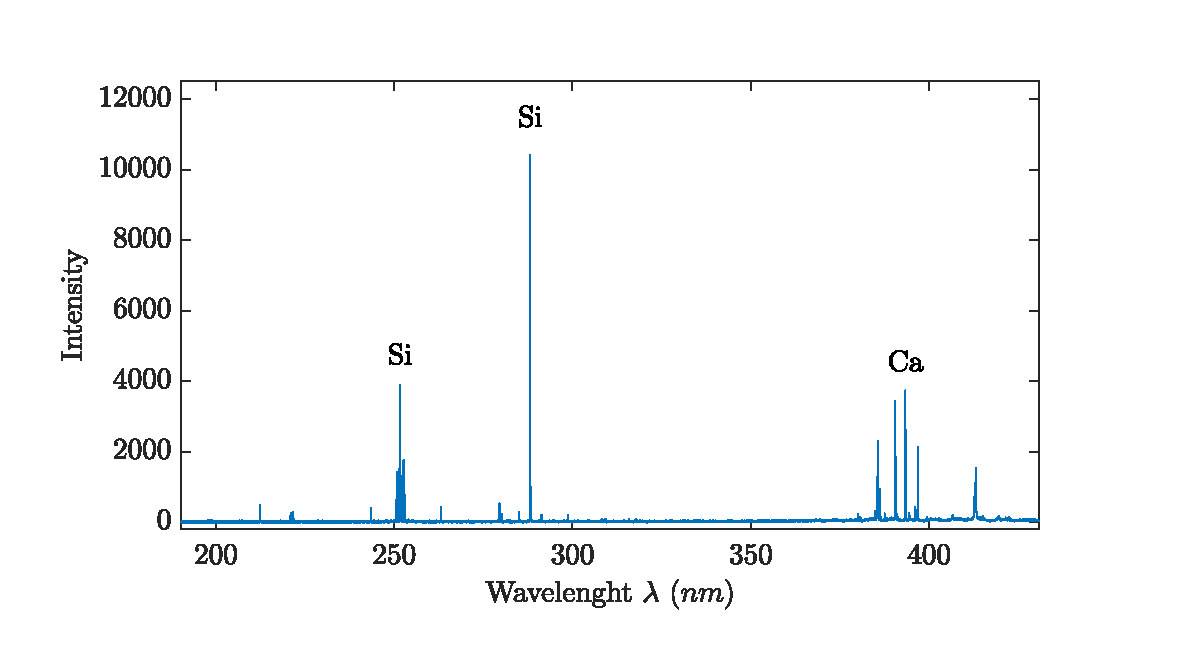
\includegraphics[width = \textwidth]{chapter_1/testFigure3.pdf}
    \label{fig:testfigure}
    \caption[Shorter caption]{Plot of the Spectra}
\end{figure}

\begin{figure}[H]
    \centering
    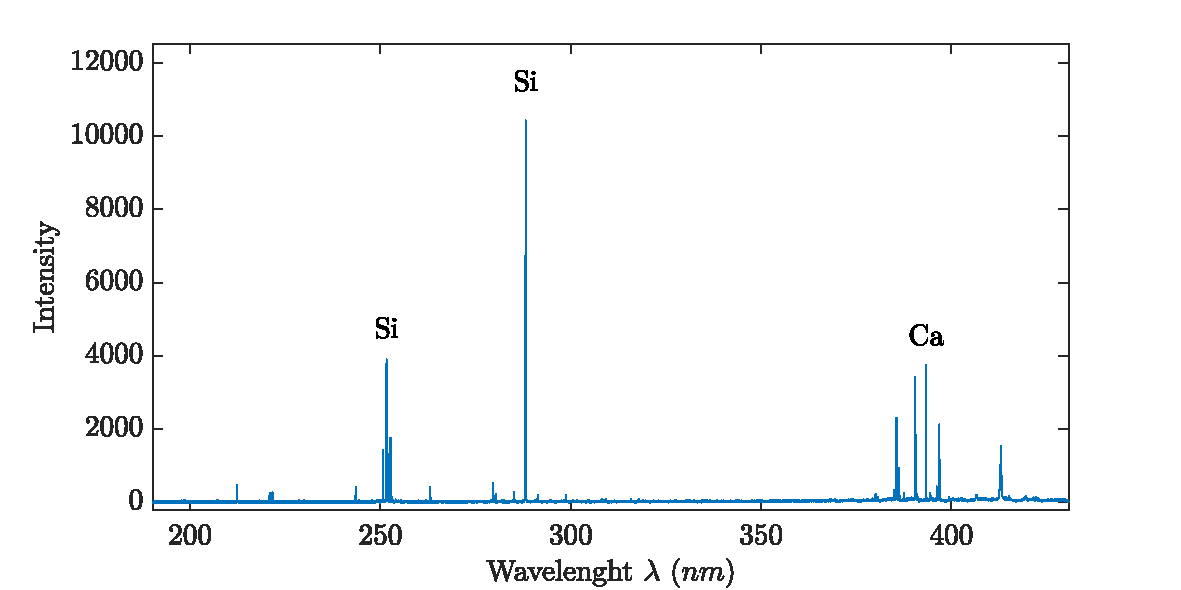
\includegraphics[width = \textwidth]{chapter_1/test_saveas2.pdf}
    \label{fig:testfigure2}
    %\caption[Shorter caption]{Plot of the Spectra}
    \caption{Plot of the Spectra}
\end{figure}



\subsection{Tables}
\label{subsec:tables}

Within the environments \texttt{table} and  \texttt{tabular} you can create very fancy tables as the one shown in Table~\ref{table:example}.
\begin{table}[H]
    \caption*{\textbf{Title of Table (optional)}}
    \centering 
    \begin{tabular}{|p{3em} c c c |}
    \hline
    \rowcolor{bluepoli!40} % comment this line to remove the color
     & \textbf{column 1} & \textbf{column 2} & \textbf{column 3} \T\B \\
    \hline \hline
    \textbf{row 1} & 1 & 2 & 3 \T\B \\
    \textbf{row 2} & $\alpha$ & $\beta$ & $\gamma$ \T\B\\
    \textbf{row 3} & alpha & beta & gamma \B\\
    \hline
    \end{tabular}
    \\[10pt]
    \caption{Caption of the Table to appear in the List of Tables.}
    \label{table:example}
\end{table}

You can also consider to highlight selected columns or rows in order to make tables more readable.
Moreover, with the use of \texttt{table*} and the option \texttt{bp} it is possible to align them at the bottom of the page. One example is presented in Table~\ref{table:exampleC}. 

\begin{table}[H]
\centering 
    \begin{tabular}{|p{3em} | c | c | c | c | c | c|}
    \hline
%    \rowcolor{bluepoli!40}
     & \textbf{column1} & \textbf{column2} & \textbf{column3} & \textbf{column4} & \textbf{column5} & \textbf{column6} \T\B \\
    \hline \hline
    \textbf{row1} & 1 & 2 & 3 & 4 & 5 & 6 \T\B\\
    \textbf{row2} & a & b & c & d & e & f \T\B\\
    \textbf{row3} & $\alpha$ & $\beta$ & $\gamma$ & $\delta$ & $\phi$ & $\omega$ \T\B\\
    \textbf{row4} & alpha & beta & gamma & delta & phi & omega \B\\
    \hline
    \end{tabular}
    \\[10pt]
    \caption{Highlighting the columns}
    \label{table:exampleC}
\end{table}

\begin{table}[H]
\centering 
    \begin{tabular}{|p{3em} c c c c c c|}
    \hline
%    \rowcolor{bluepoli!40}
     & \textbf{column1} & \textbf{column2} & \textbf{column3} & \textbf{column4} & \textbf{column5} & \textbf{column6} \T\B \\
    \hline \hline
    \textbf{row1} & 1 & 2 & 3 & 4 & 5 & 6 \T\B\\
    \hline
    \textbf{row2} & a & b & c & d & e & f \T\B\\
    \hline
    \textbf{row3} & $\alpha$ & $\beta$ & $\gamma$ & $\delta$ & $\phi$ & $\omega$ \T\B\\
    \hline
    \textbf{row4} & alpha & beta & gamma & delta & phi & omega \B\\
    \hline
    \end{tabular}
    \\[10pt]
    \caption{Highlighting the rows}
    \label{table:exampleR}
\end{table}

\subsection{Algorithms}
\label{subsec:algorithms}

Pseudo-algorithms can be written in \LaTeX{} with the \texttt{algorithm} and \texttt{algorithmic} packages.
An example is shown in Algorithm~\ref{alg:var}.
\begin{algorithm}[H]
    \label{alg:example}
    \caption{Name of the Algorithm}
    \label{alg:var}
    \label{protocol1}
    \begin{algorithmic}[1]
    \STATE Initial instructions
    \FOR{$for-condition$}
    \STATE{Some instructions}
    \IF{$if-condition$}
    \STATE{Some other instructions}
    \ENDIF
    \ENDFOR
    \WHILE{$while-condition$}
    \STATE{Some further instructions}
    \ENDWHILE
    \STATE Final instructions
    \end{algorithmic}
\end{algorithm} 

\vspace{5mm}

\section{Theorems, propositions and lists}

\subsection{Theorems}
Theorems have to be formatted as:
\begin{theorem}
\label{a_theorem}
Write here your theorem. 
\end{theorem}
\textit{Proof.} If useful you can report here the proof.

\subsection{Propositions}
Propositions have to be formatted as:
\begin{proposition}
Write here your proposition.
\end{proposition}

\subsection{Lists}
How to  insert itemized lists:
\begin{itemize}
    \item first item;
    \item second item.
\end{itemize}
How to insert numbered lists:
\begin{enumerate}
    \item first item;
    \item second item.
\end{enumerate}

\section{Use of copyrighted material}

Each student is responsible for obtaining copyright permissions, if necessary, to include published material in the thesis.
This applies typically to third-party material published by someone else.

\section{Plagiarism}

You have to be sure to respect the rules on Copyright and avoid an involuntary plagiarism.
It is allowed to take other persons' ideas only if the author and his original work are clearly mentioned.
As stated in the Code of Ethics and Conduct, Politecnico di Milano \textit{promotes the integrity of research,
condemns manipulation and the infringement of intellectual property}, and gives opportunity to all those
who carry out research activities to have an adequate training on ethical conduct and integrity while doing research.
To be sure to respect the copyright rules, read the guides on Copyright legislation and citation styles available
at:
\begin{verbatim}
https://www.biblio.polimi.it/en/tools/courses-and-tutorials
\end{verbatim}
You can also attend the courses which are periodically organized on "Bibliographic citations and bibliography management".

\section{Bibliography and citations}
Your thesis must contain a suitable Bibliography which lists all the sources consulted on developing the work.
The list of references is placed at the end of the manuscript after the chapter containing the conclusions.
We suggest to use the BibTeX package and save the bibliographic references  in the file \verb|Thesis_bibliography.bib|.
This is indeed a database containing all the information about the references. To cite in your manuscript, use the \verb|\cite{}| command as follows:
\\
\textit{Here is how you cite bibliography entries: \cite{knuth74}, or multiple ones at once: \cite{knuth92,lamport94}}.
\\
The bibliography and list of references are generated automatically by running BibTeX \cite{bibtex}.

\chapter{Conclusions and future developments}
\label{ch:conclusions}%
A final chapter containing the main conclusions of your research/study
and possible future developments of your work have to be inserted in this chapter.

%-------------------------------------------------------------------------
%	BIBLIOGRAPHY
%-------------------------------------------------------------------------

\addtocontents{toc}{\vspace{2em}} % Add a gap in the Contents, for aesthetics
\bibliography{Thesis_bibliography} % The references information are stored in the file named "Thesis_bibliography.bib"

%-------------------------------------------------------------------------
%	APPENDICES
%-------------------------------------------------------------------------

\cleardoublepage
\addtocontents{toc}{\vspace{2em}} % Add a gap in the Contents, for aesthetics
\appendix
\chapter{Appendix A}
If you need to include an appendix to support the research in your thesis, you can place it at the end of the manuscript.
An appendix contains supplementary material (figures, tables, data, codes, mathematical proofs, surveys, \dots)
which supplement the main results contained in the previous chapters.

\chapter{Appendix B}
It may be necessary to include another appendix to better organize the presentation of supplementary material.


% LIST OF FIGURES
\listoffigures

% LIST OF TABLES
\listoftables

% LIST OF SYMBOLS
% Write out the List of Symbols in this page
\chapter*{List of Symbols} % You have to include a chapter for your list of symbols (
\begin{table}[H]
    \centering
    \begin{tabular}{lll}
        \textbf{Variable} & \textbf{Description} & \textbf{SI unit} \\\hline\\[-9px]
        $\bm{u}$ & solid displacement & m \\[2px]
        $\bm{u}_f$ & fluid displacement & m \\[2px]
    \end{tabular}
\end{table}

% ACKNOWLEDGEMENTS
\chapter*{Acknowledgements}
Here you might want to acknowledge someone.

\cleardoublepage

\end{document}
